\documentclass[
	12pt,twoside,a4paper
]{report}

\usepackage{graphicx}
\usepackage[margin=1in]{geometry}
\usepackage{fancyhdr}
\usepackage[utf8]{inputenc}
\usepackage{etoc}
\usepackage{xcolor, soul}
\usepackage{listings}
\usepackage{amsmath}
\usepackage{lipsum}
\usepackage{pgfplots}
\usepackage{hyperref}
\usepackage{circuitikz}
\usepackage{caption}
\usepackage{subcaption}
\usepackage[table,xcdraw]{xcolor}

\sethlcolor{yellow}

\fancypagestyle{plain}{
	\fancyhf{}
	\fancyhead[l]{Lab Experiment \#4}
	\fancyhead[c]{Operational Amplifiers}
	\fancyhead[r]{May 25, 2024}
	\fancyfoot[le, ro]{Page \thepage}
	\fancyfoot[re, lo]{ESD Capsule 2024}
	\fancyfoot[c]{EE211}
	\setlength{\headheight}{15pt}
	\renewcommand{\headrulewidth}{0.2pt}
	\renewcommand{\footrulewidth}{0.2pt}
}	

\thispagestyle{plain}

\renewcommand{\etocaftertitlehook}{\thispagestyle{plain}}
\renewcommand{\etocaftertochook}{\thispagestyle{plain}}

\begin{document}
	\begin{center}
	
\includegraphics[width=0.4\textwidth]{assets/agu.png}

	\Huge
	\textbf{\paperTitle}

	\vspace{0.3cm}
	\Huge
	\paperSubTitle{}

	\vspace{0.8cm}
	\large
	\vspace{0.5cm}
	\LARGE
	\vspace{1.5cm}
	\textbf{}
	\vfill
	\vspace{0.8cm}
	\Large
\end{center}

\begin{tabbing}
	\hspace*{1em}\= \hspace*{8em} \= \kill
	\> \author{} \> \sid{} \\
	\> \> \\
	\> April 23, 2024 \> \\
\end{tabbing}

	\tableofcontents

	\chapter{Introduction}

The aim of this lab work is to familiarize ourselves with Operational Amplifiers (Op-Amps). This includes theoretical analysis, simulation using LTspice, and practical implementation to observe the behavior of inverting and non-inverting Op-Amps under various conditions.

	\chapter{Theoretical Analysis}

\section{Circuit 1: Non-Inverting Amplifier}

\begin{figure}[h]
    \centering
    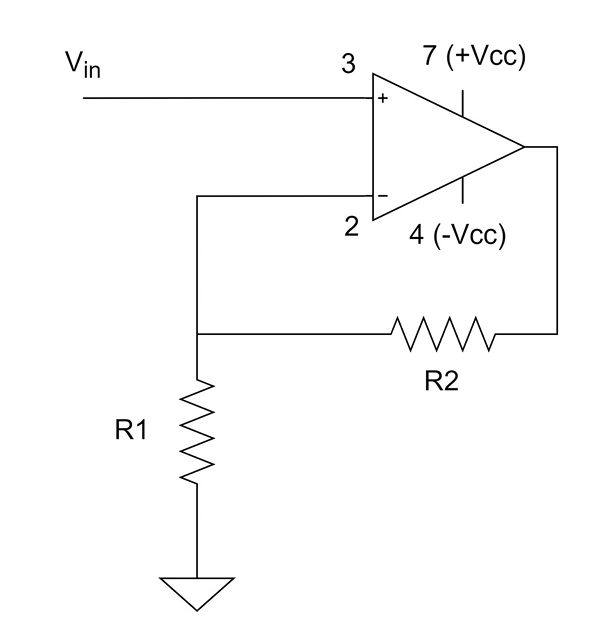
\includegraphics[width=0.5\textwidth]{assets/non-inverting.png}
    \caption{Non-Inverting Amplifier}
    \label{fig:non-inverting-amplifier}
\end{figure}

The non-inverting amplifier is a type of operational amplifier circuit that uses positive feedback to provide a closed-loop gain. The circuit is shown in Figure \ref{fig:non-inverting-amplifier}. The gain of the non-inverting amplifier is given by the formula:

\begin{equation}
    A = 1 + \frac{R_2}{R_1}
\end{equation}

In our case, $f = 1kHz$, $V_{in} = 100mV$, $R_1 = 1k\Omega$ and $R_2 = 22k\Omega$. Therefore, the gain of the non-inverting amplifier is:

\begin{equation}
    A = 1 + \frac{22k\Omega}{1k\Omega} = 23
\end{equation}

\noindent And expected output is calculated as:

\begin{equation}
    V_{out} = A \cdot V_{in} = 23 \cdot 100mV = 2.3V
\end{equation}

\newpage
\thispagestyle{plain}

\section{Circuit 2: Inverting Amplifier}

\begin{figure}[h]
    \centering
    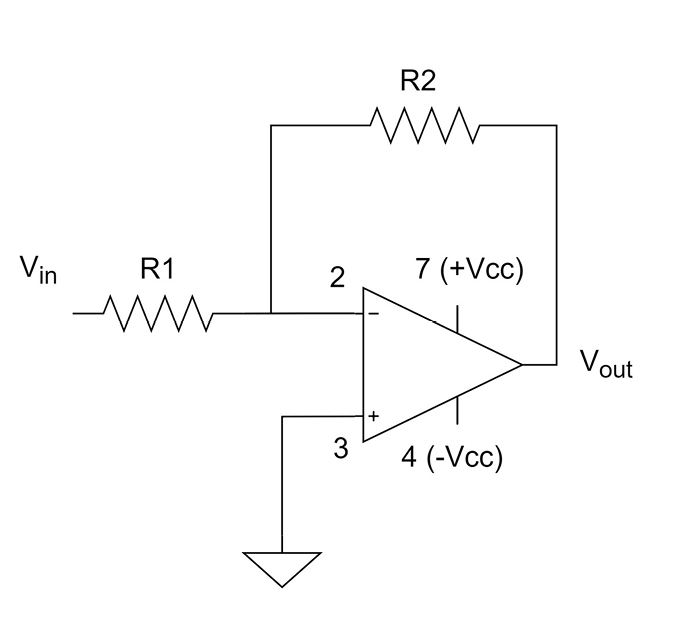
\includegraphics[width=0.5\textwidth]{assets/inverting.png}
    \caption{Inverting Amplifier}
    \label{fig:inverting-amplifier}
\end{figure}

Every calculation is similar to the non-inverting amplifier, except the gain formula. The gain of the inverting amplifier is:

\begin{equation}
    A = -\frac{R_2}{R_1}
\end{equation}

In our case, $f = 1kHz$, $V_{in} = 100mV$, $R_1 = 1k\Omega$ and $R_2 = 22k\Omega$. Therefore, the gain of the inverting amplifier is:

\begin{equation}
    A = -\frac{22k\Omega}{1k\Omega} = -22
\end{equation}

\noindent And expected output is calculated as:

\begin{equation}
    V_{out} = A \cdot V_{in} = -22 \cdot 100mV = -2.2V
\end{equation}

\newpage
\thispagestyle{plain}

\section{LTspice Simulation}

\subsection{Non-Inverting Amplifier}

\begin{figure}[h]
    \centering
    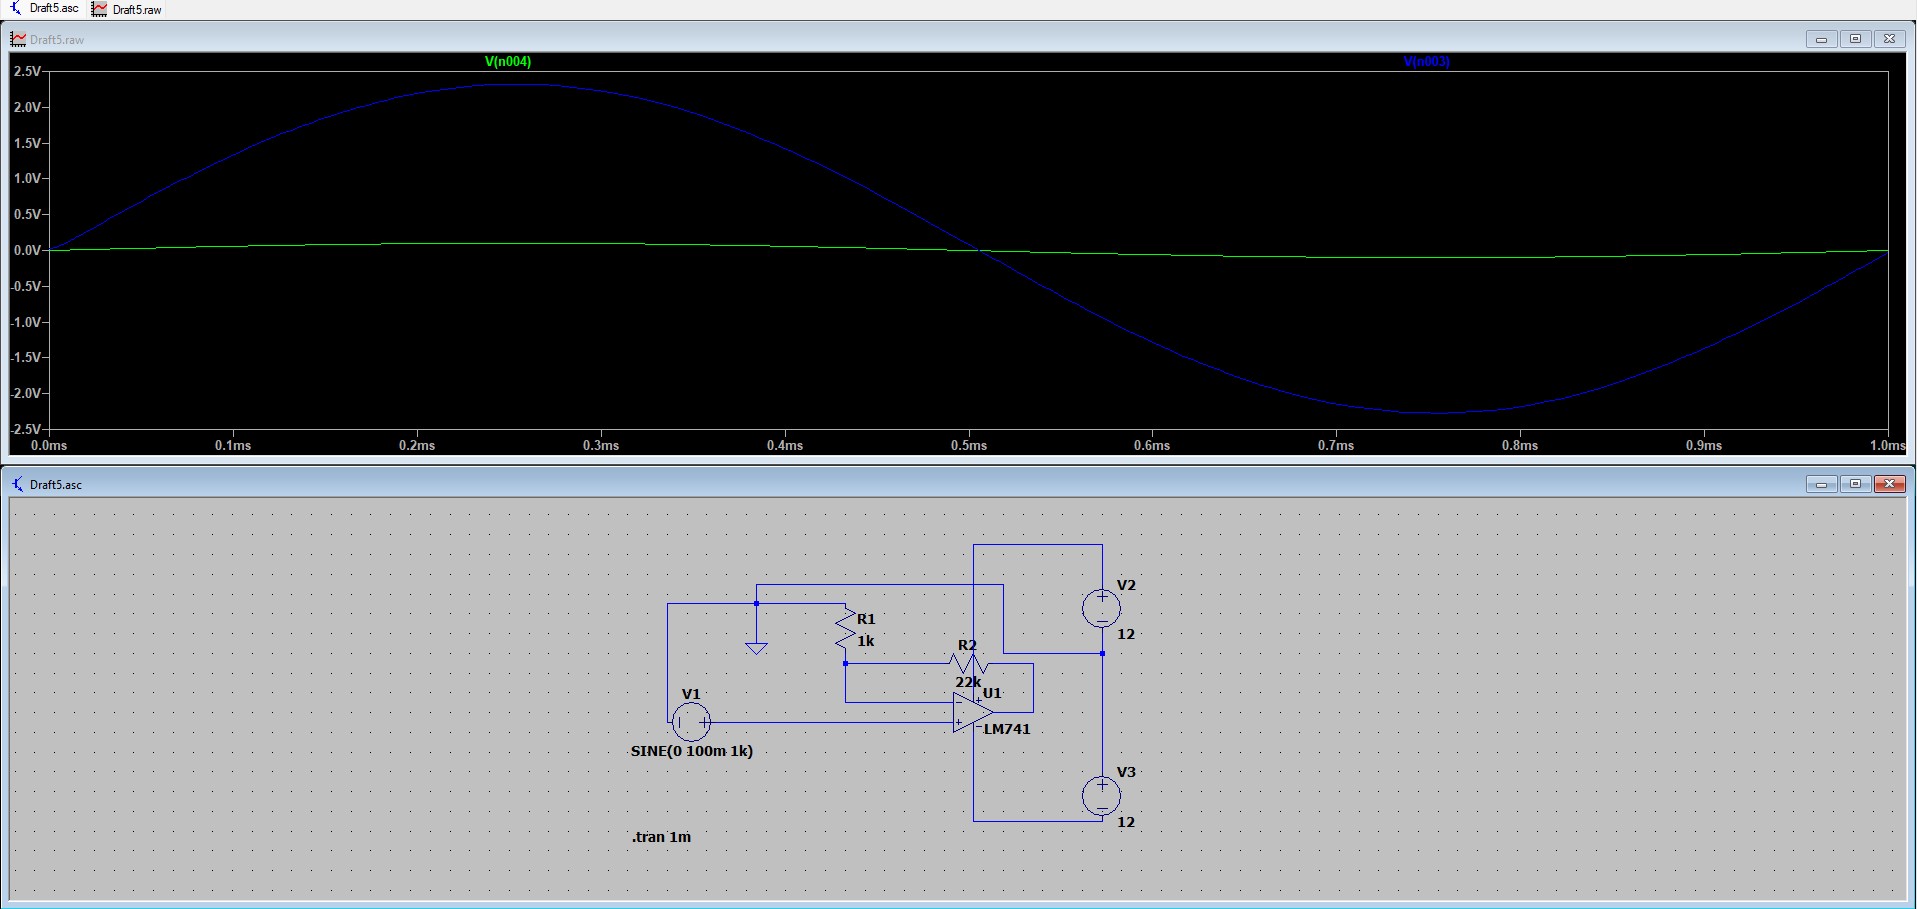
\includegraphics[width=1\textwidth]{assets/100m-non-inverting.png}
    \caption{Non-Inverting Amplifier @ 100mV}
    \label{fig:100m-non-inverting}
\end{figure}

Applying 100mV input to the non-inverting amplifier, the output is 2.3V as expected. The simulation result is shown in Figure \ref{fig:100m-non-inverting}. 

\begin{figure}[h]
    \centering
    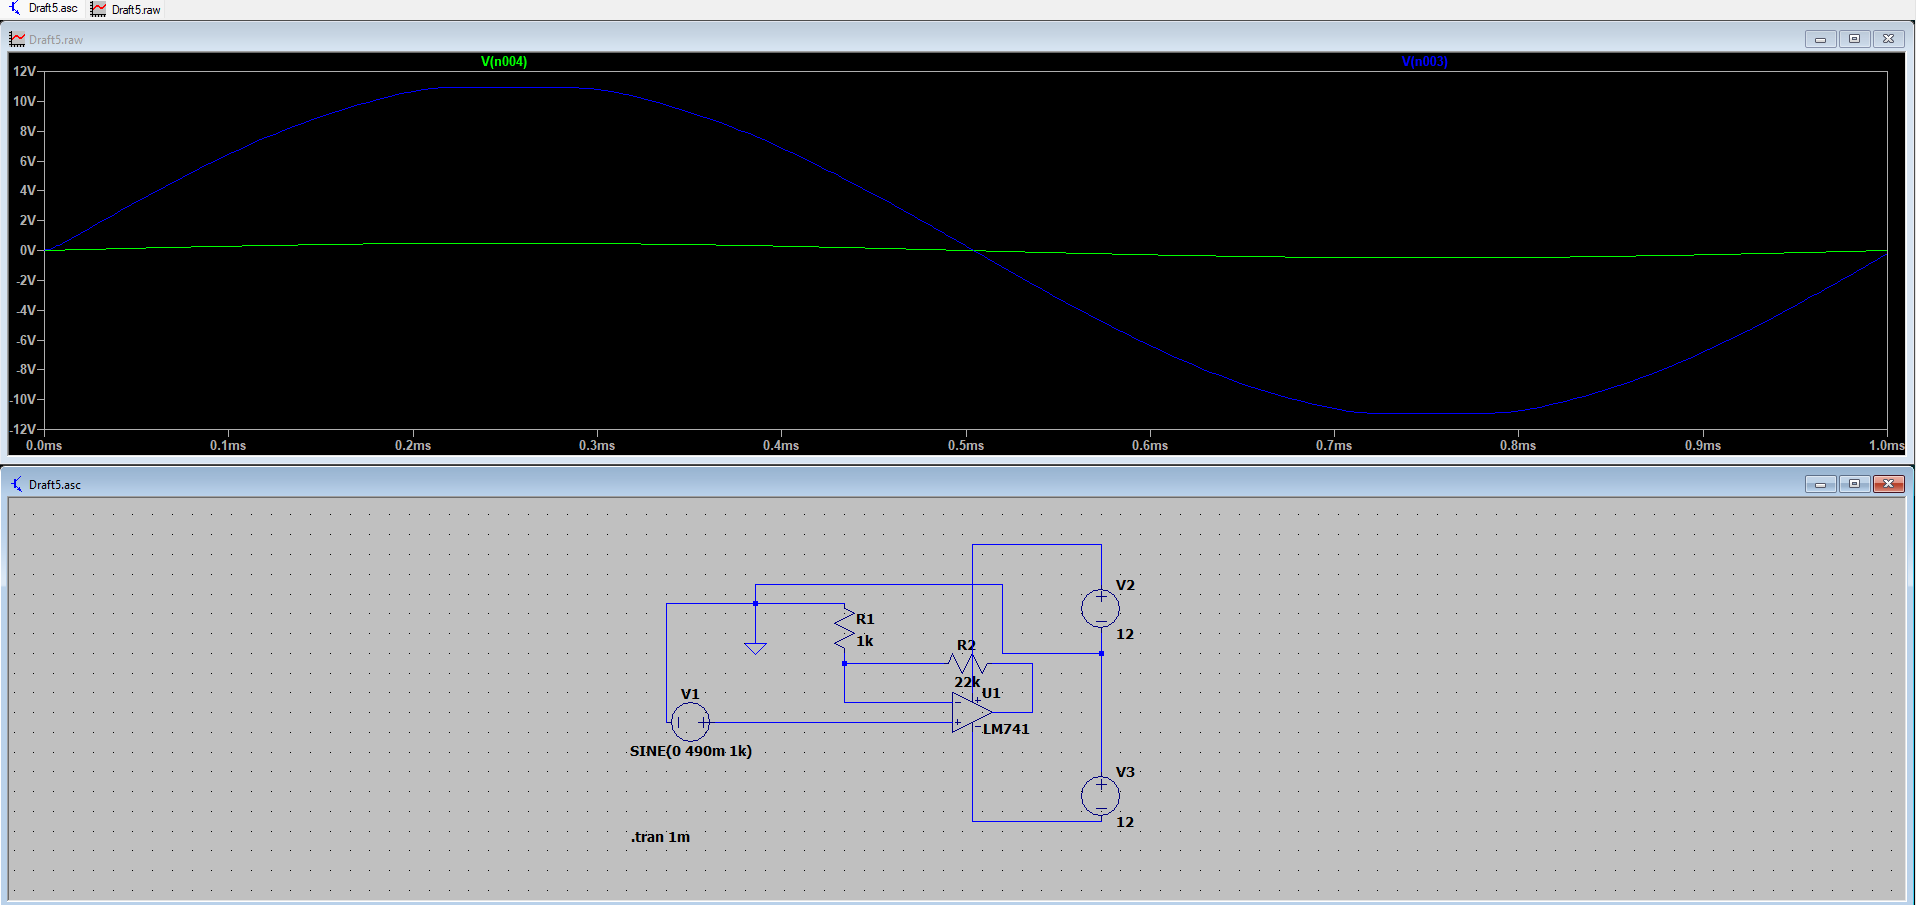
\includegraphics[width=1\textwidth]{assets/490m-non-inverting.png}
    \caption{Non-Inverting Amplifier @ 490mV}
    \label{fig:490m-non-inverting}
\end{figure}

Applying 490mV input to the non-inverting amplifier, the output should be 13.7V but it is limited to 12V due to the power supply as seen in Figure \ref{fig:490m-non-inverting}.

\newpage
\thispagestyle{plain}

\begin{figure}[h]
    \centering
    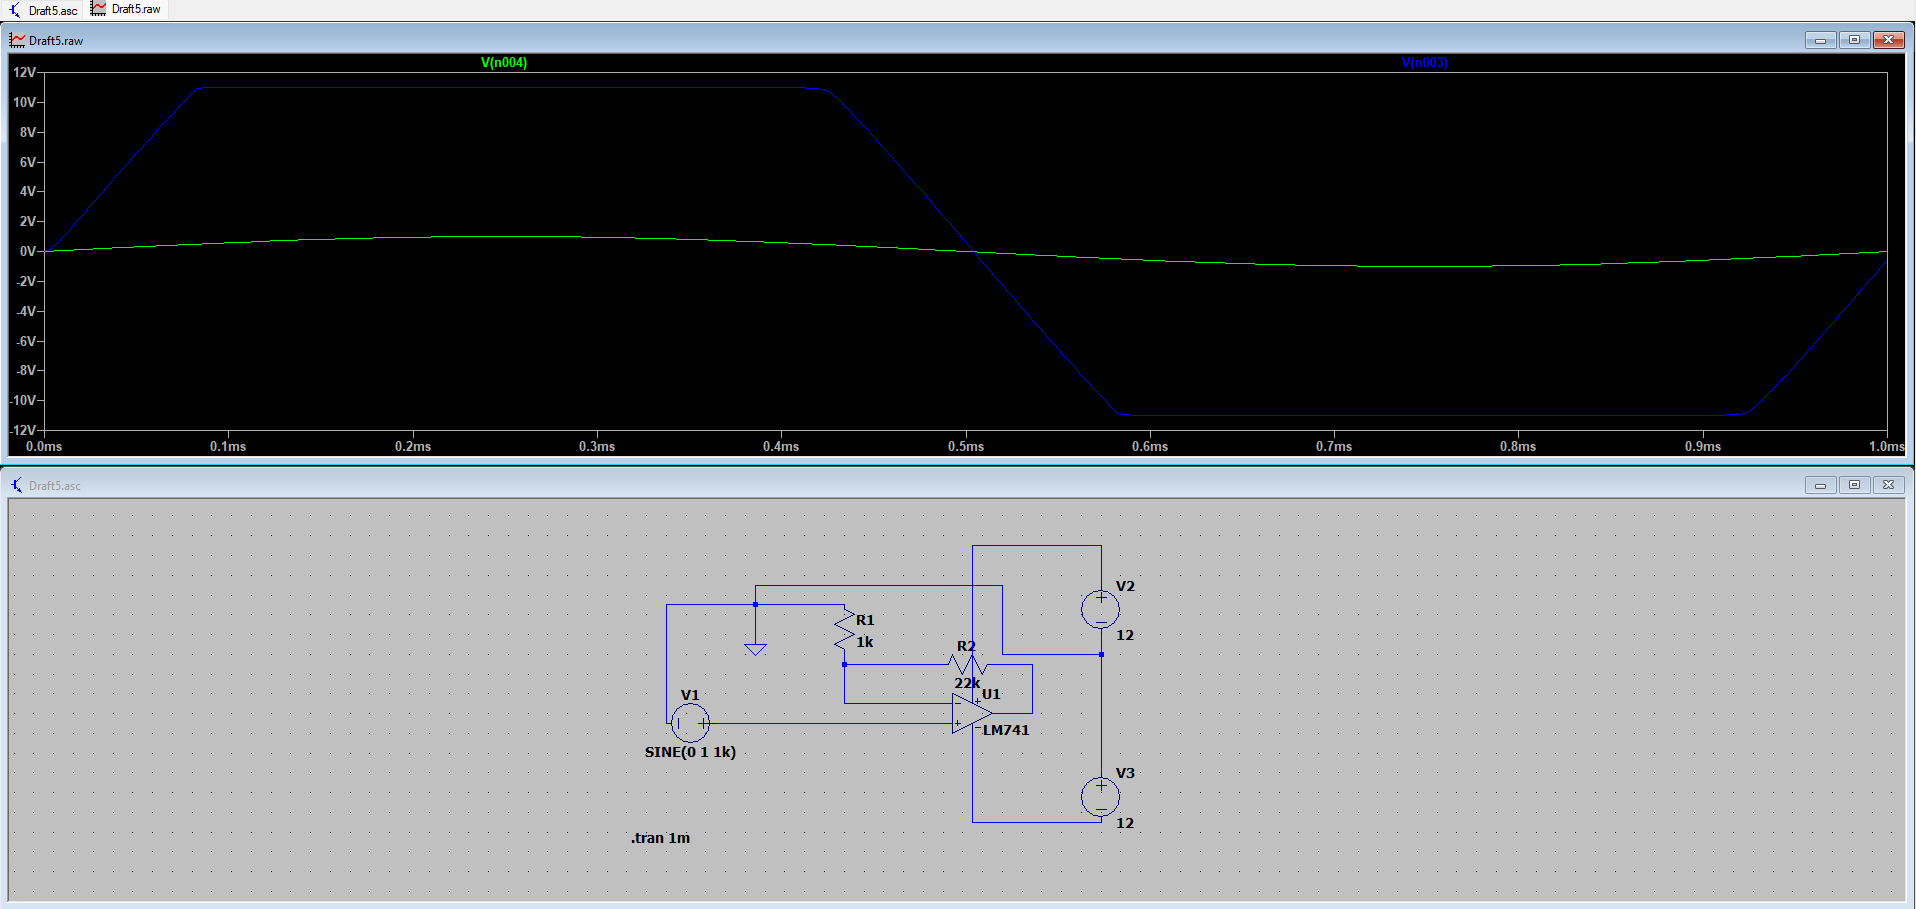
\includegraphics[width=1\textwidth]{assets/1-non-inverting.png}
    \caption{Non-Inverting Amplifier @ 1V}
    \label{fig:1-non-inverting}
\end{figure}

Applying 1V input to the non-inverting amplifier, the output should be 23V but it is limited to 12V due to the power supply as it is \textbf{more visible} in Figure \ref{fig:1-non-inverting}.

\newpage
\thispagestyle{plain}

\subsection{Inverting Amplifier}

\begin{figure}[h]
    \centering
    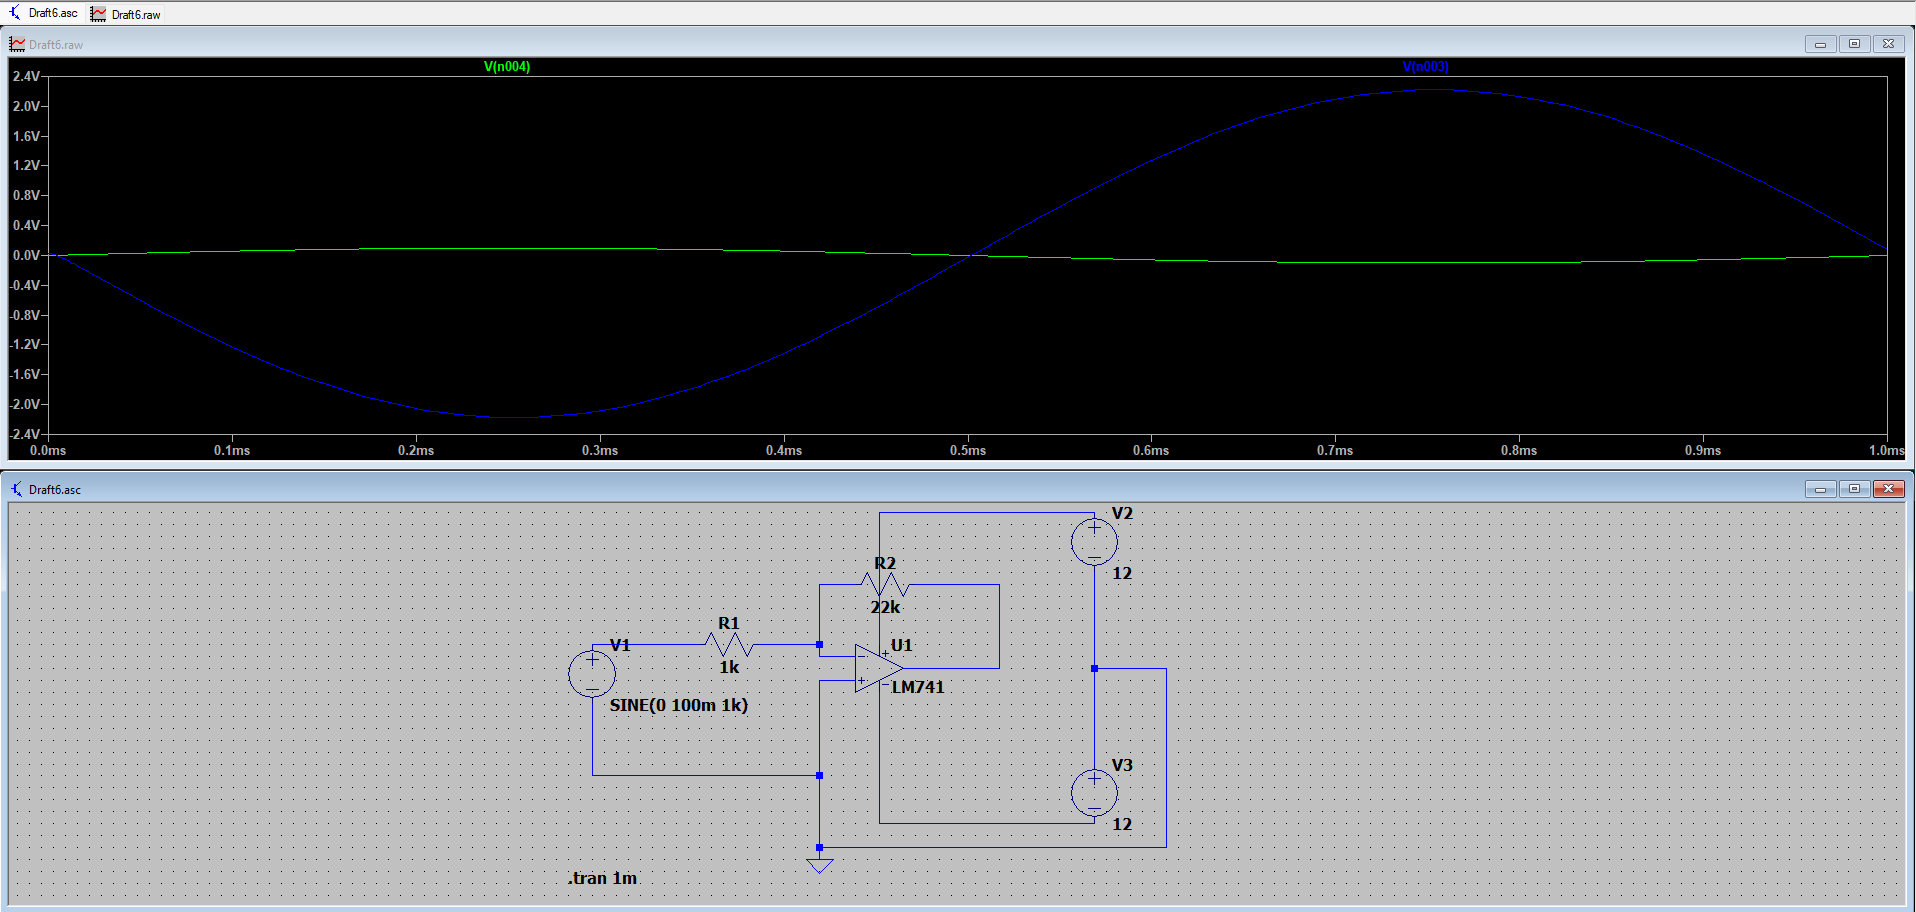
\includegraphics[width=1\textwidth]{assets/100m-inverting.png}
    \caption{Inverting Amplifier @ 100mV}
    \label{fig:100m-inverting}
\end{figure}

Applying 100mV input to the inverting amplifier, the output is -2.2V as expected. The simulation result is shown in Figure \ref{fig:100m-inverting}.

\begin{figure}[h]
    \centering
    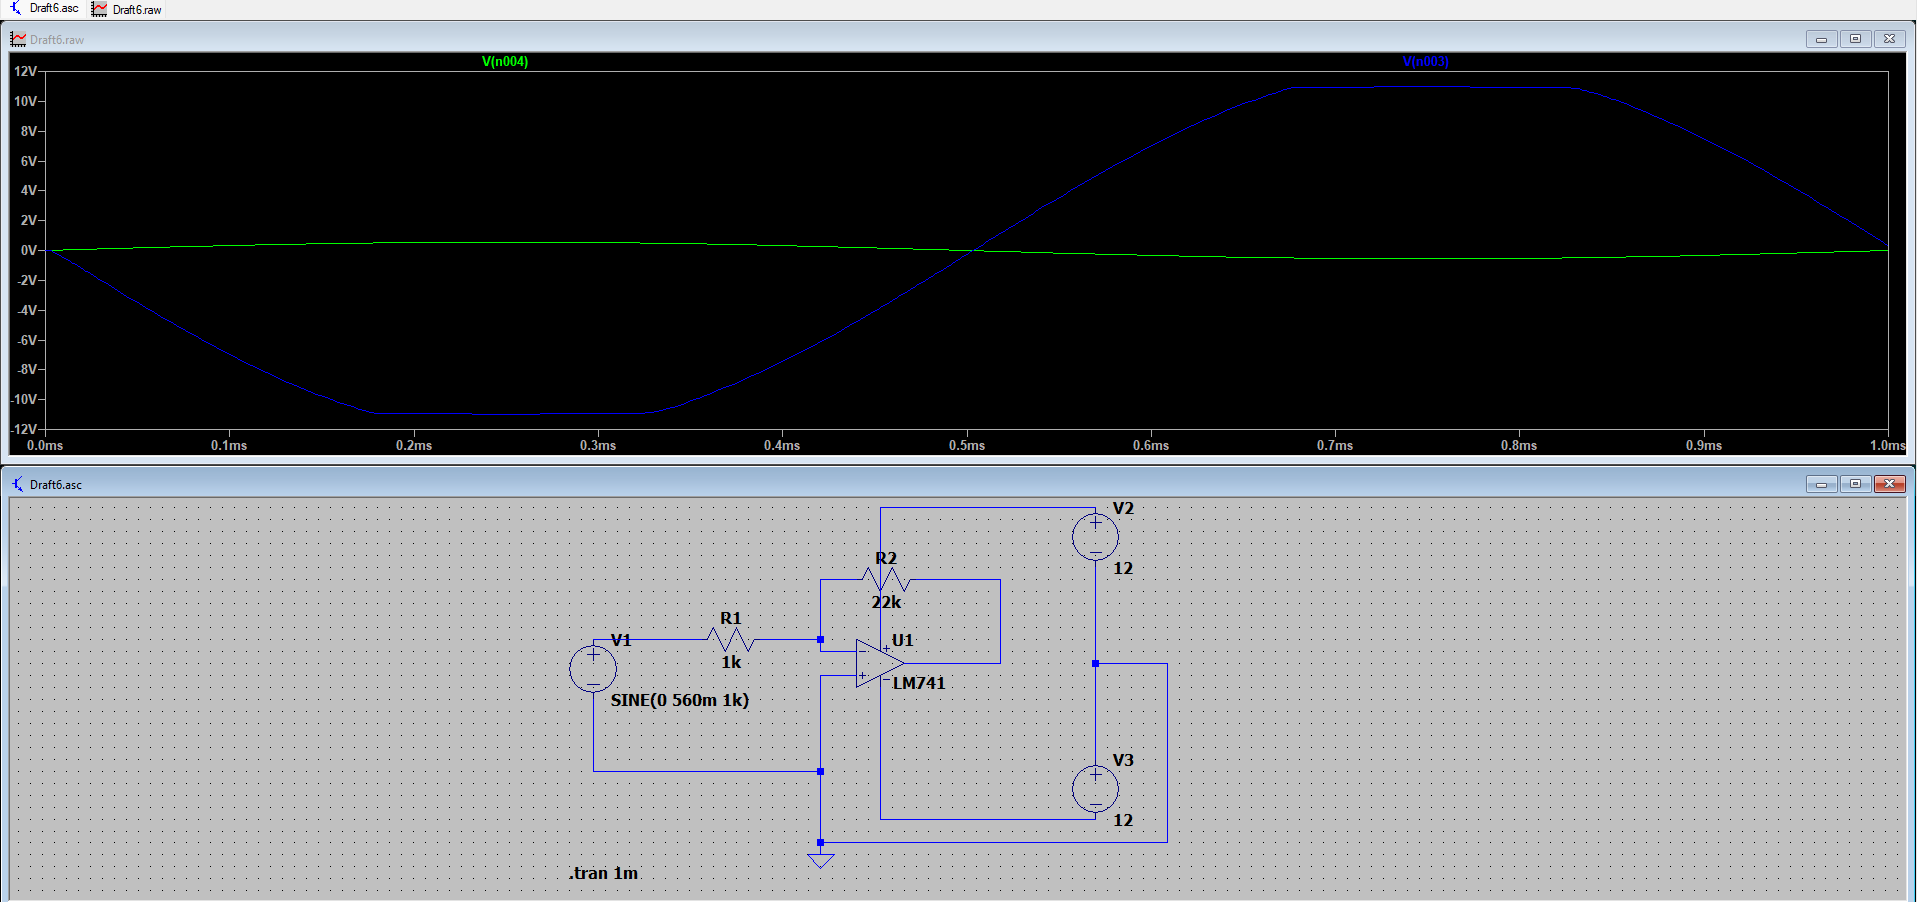
\includegraphics[width=1\textwidth]{assets/560m-inverting.png}
    \caption{Inverting Amplifier @ 560mV}
    \label{fig:560m-inverting}
\end{figure}

Applying 560mV input to the inverting amplifier, the output should be -12.32V but it is limited to -12V due to the power supply as seen in Figure \ref{fig:560m-inverting}.

\newpage
\thispagestyle{plain}

\begin{figure}[h]
    \centering
    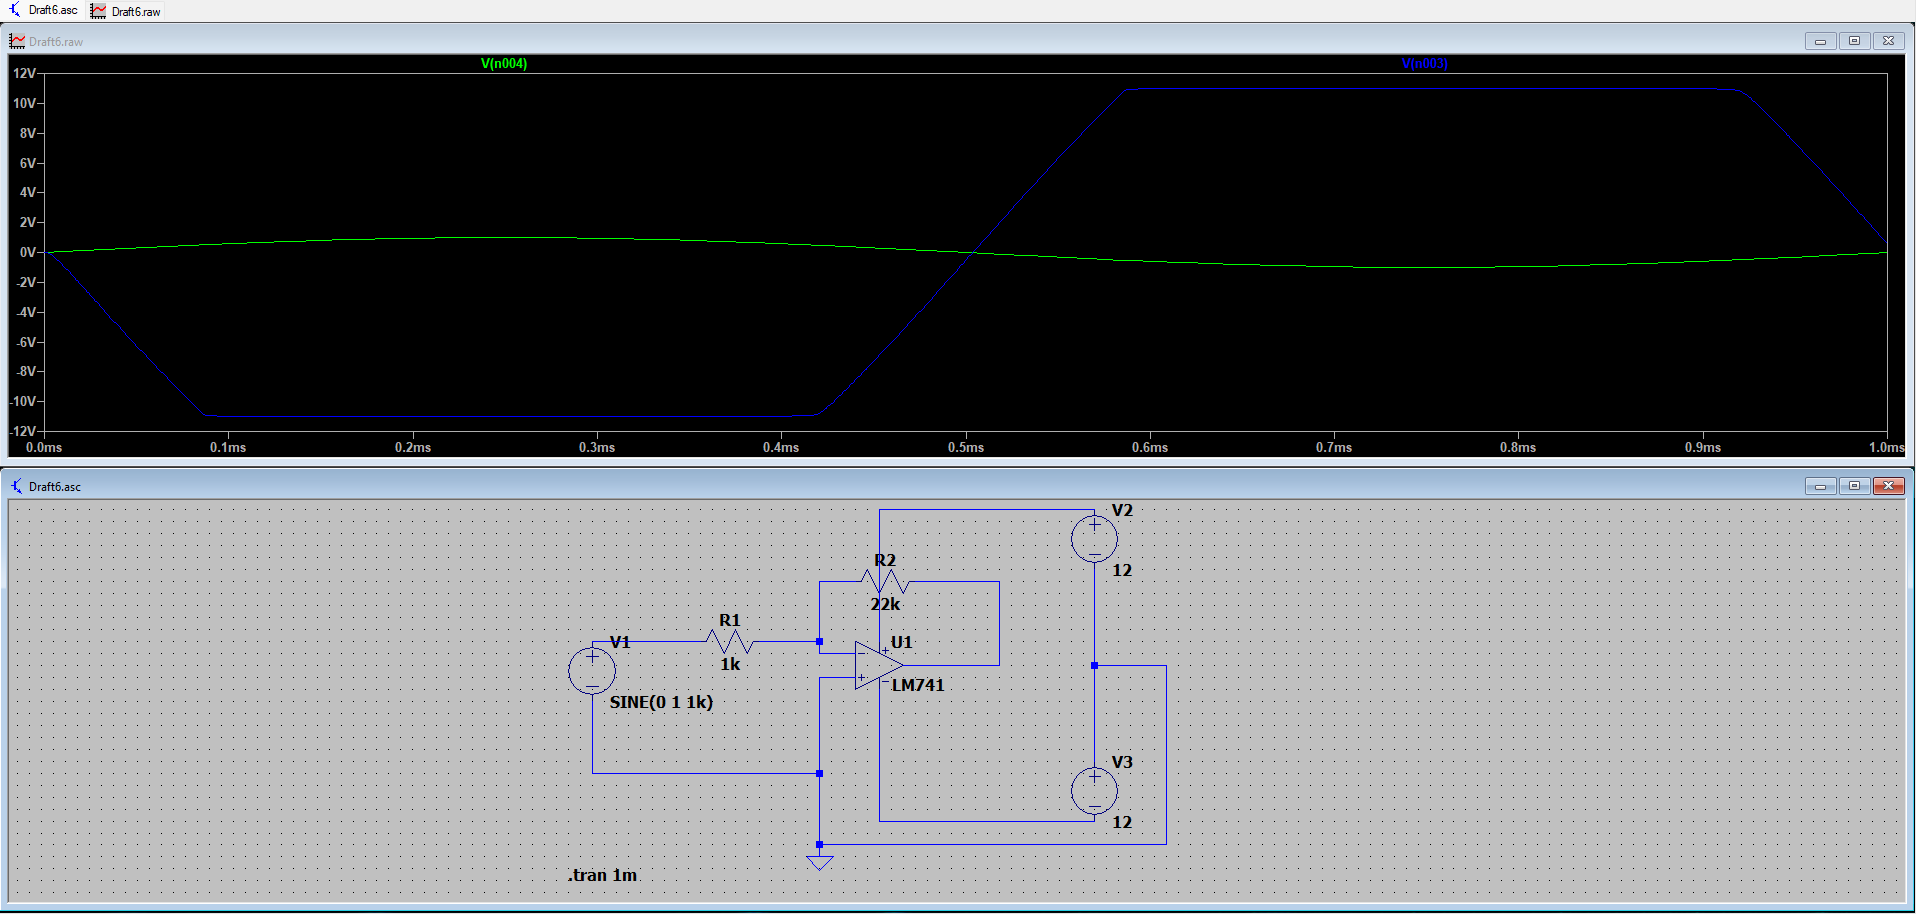
\includegraphics[width=1\textwidth]{assets/1-inverting.png}
    \caption{Inverting Amplifier @ 1V}
    \label{fig:1-inverting}
\end{figure}

Applying 1V input to the inverting amplifier, the output should be -22V but it is limited to -12V due to the power supply as it is \textbf{more visible} in Figure \ref{fig:1-inverting}.


	\chapter{Experimental Results}

\section{Circuit Construction}

\subsection{Non-Inverting Amplifier}

\begin{figure}[h]
    \centering
    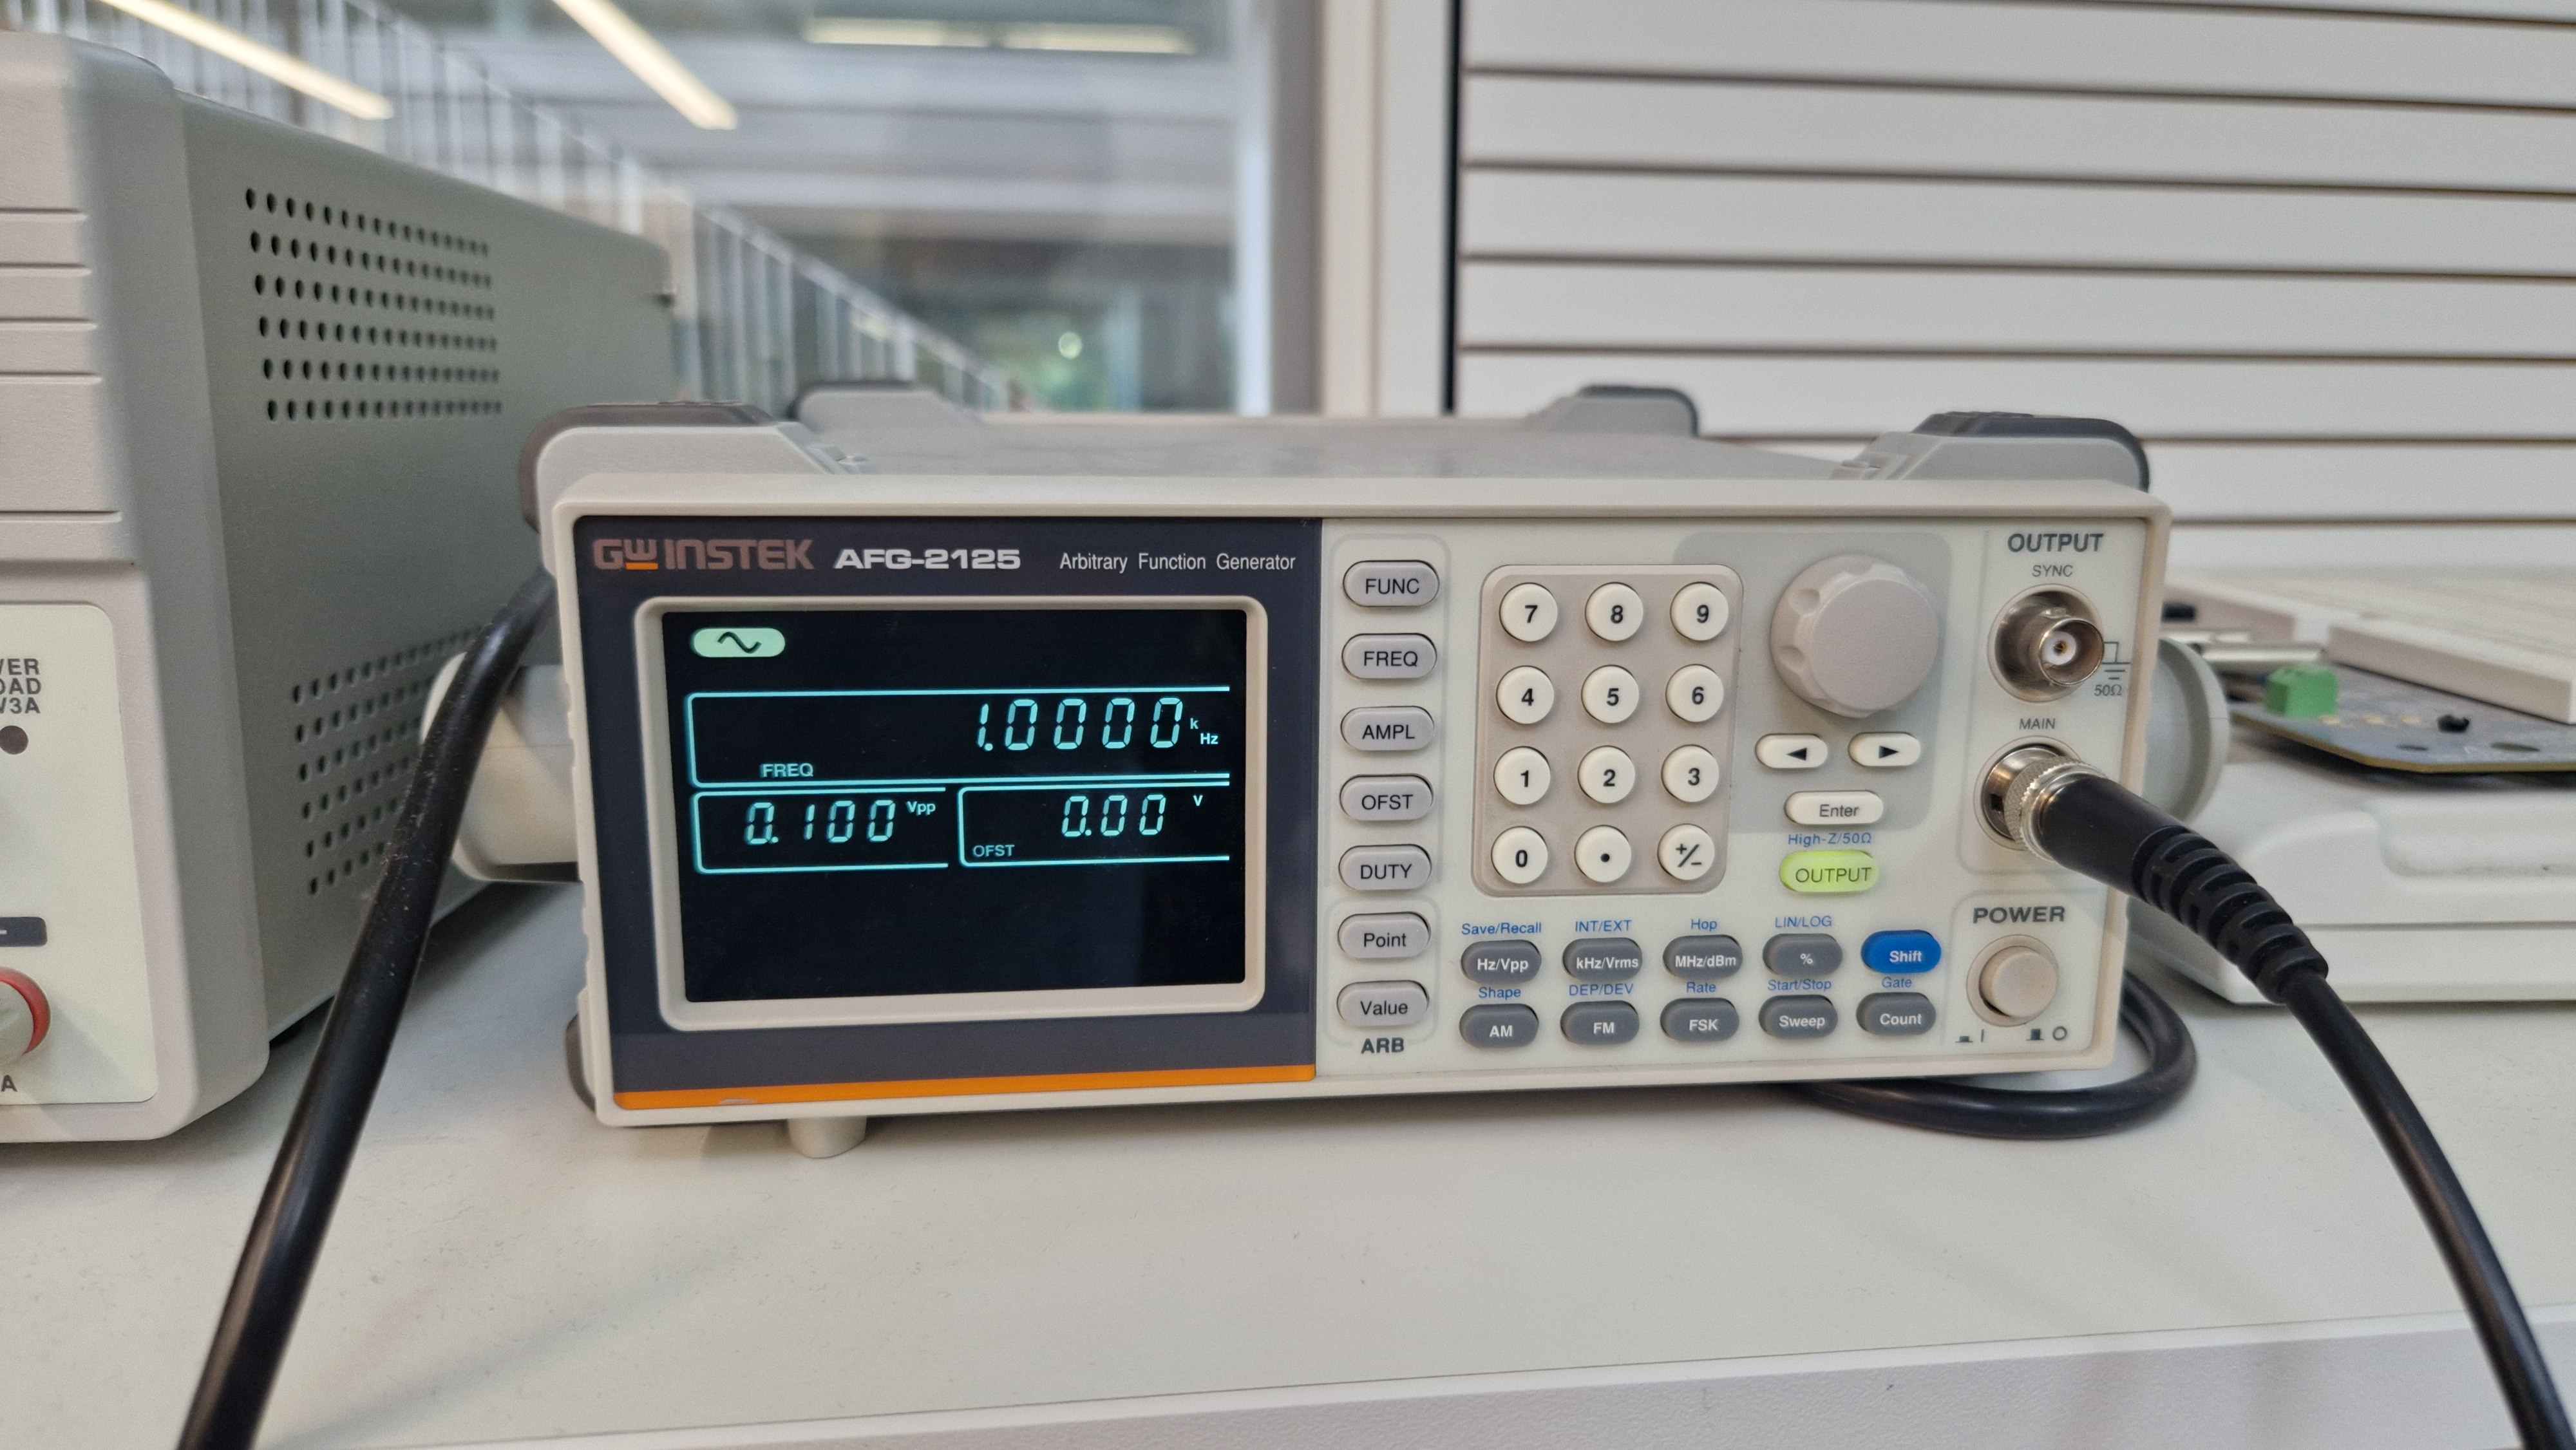
\includegraphics[width=0.6\textwidth]{assets/non-inverting-100m.jpg}
    \caption{Signal Generator @ 100mV}
    \label{fig:non-inverting-100m}
\end{figure}

\begin{figure}[h]
    \centering
    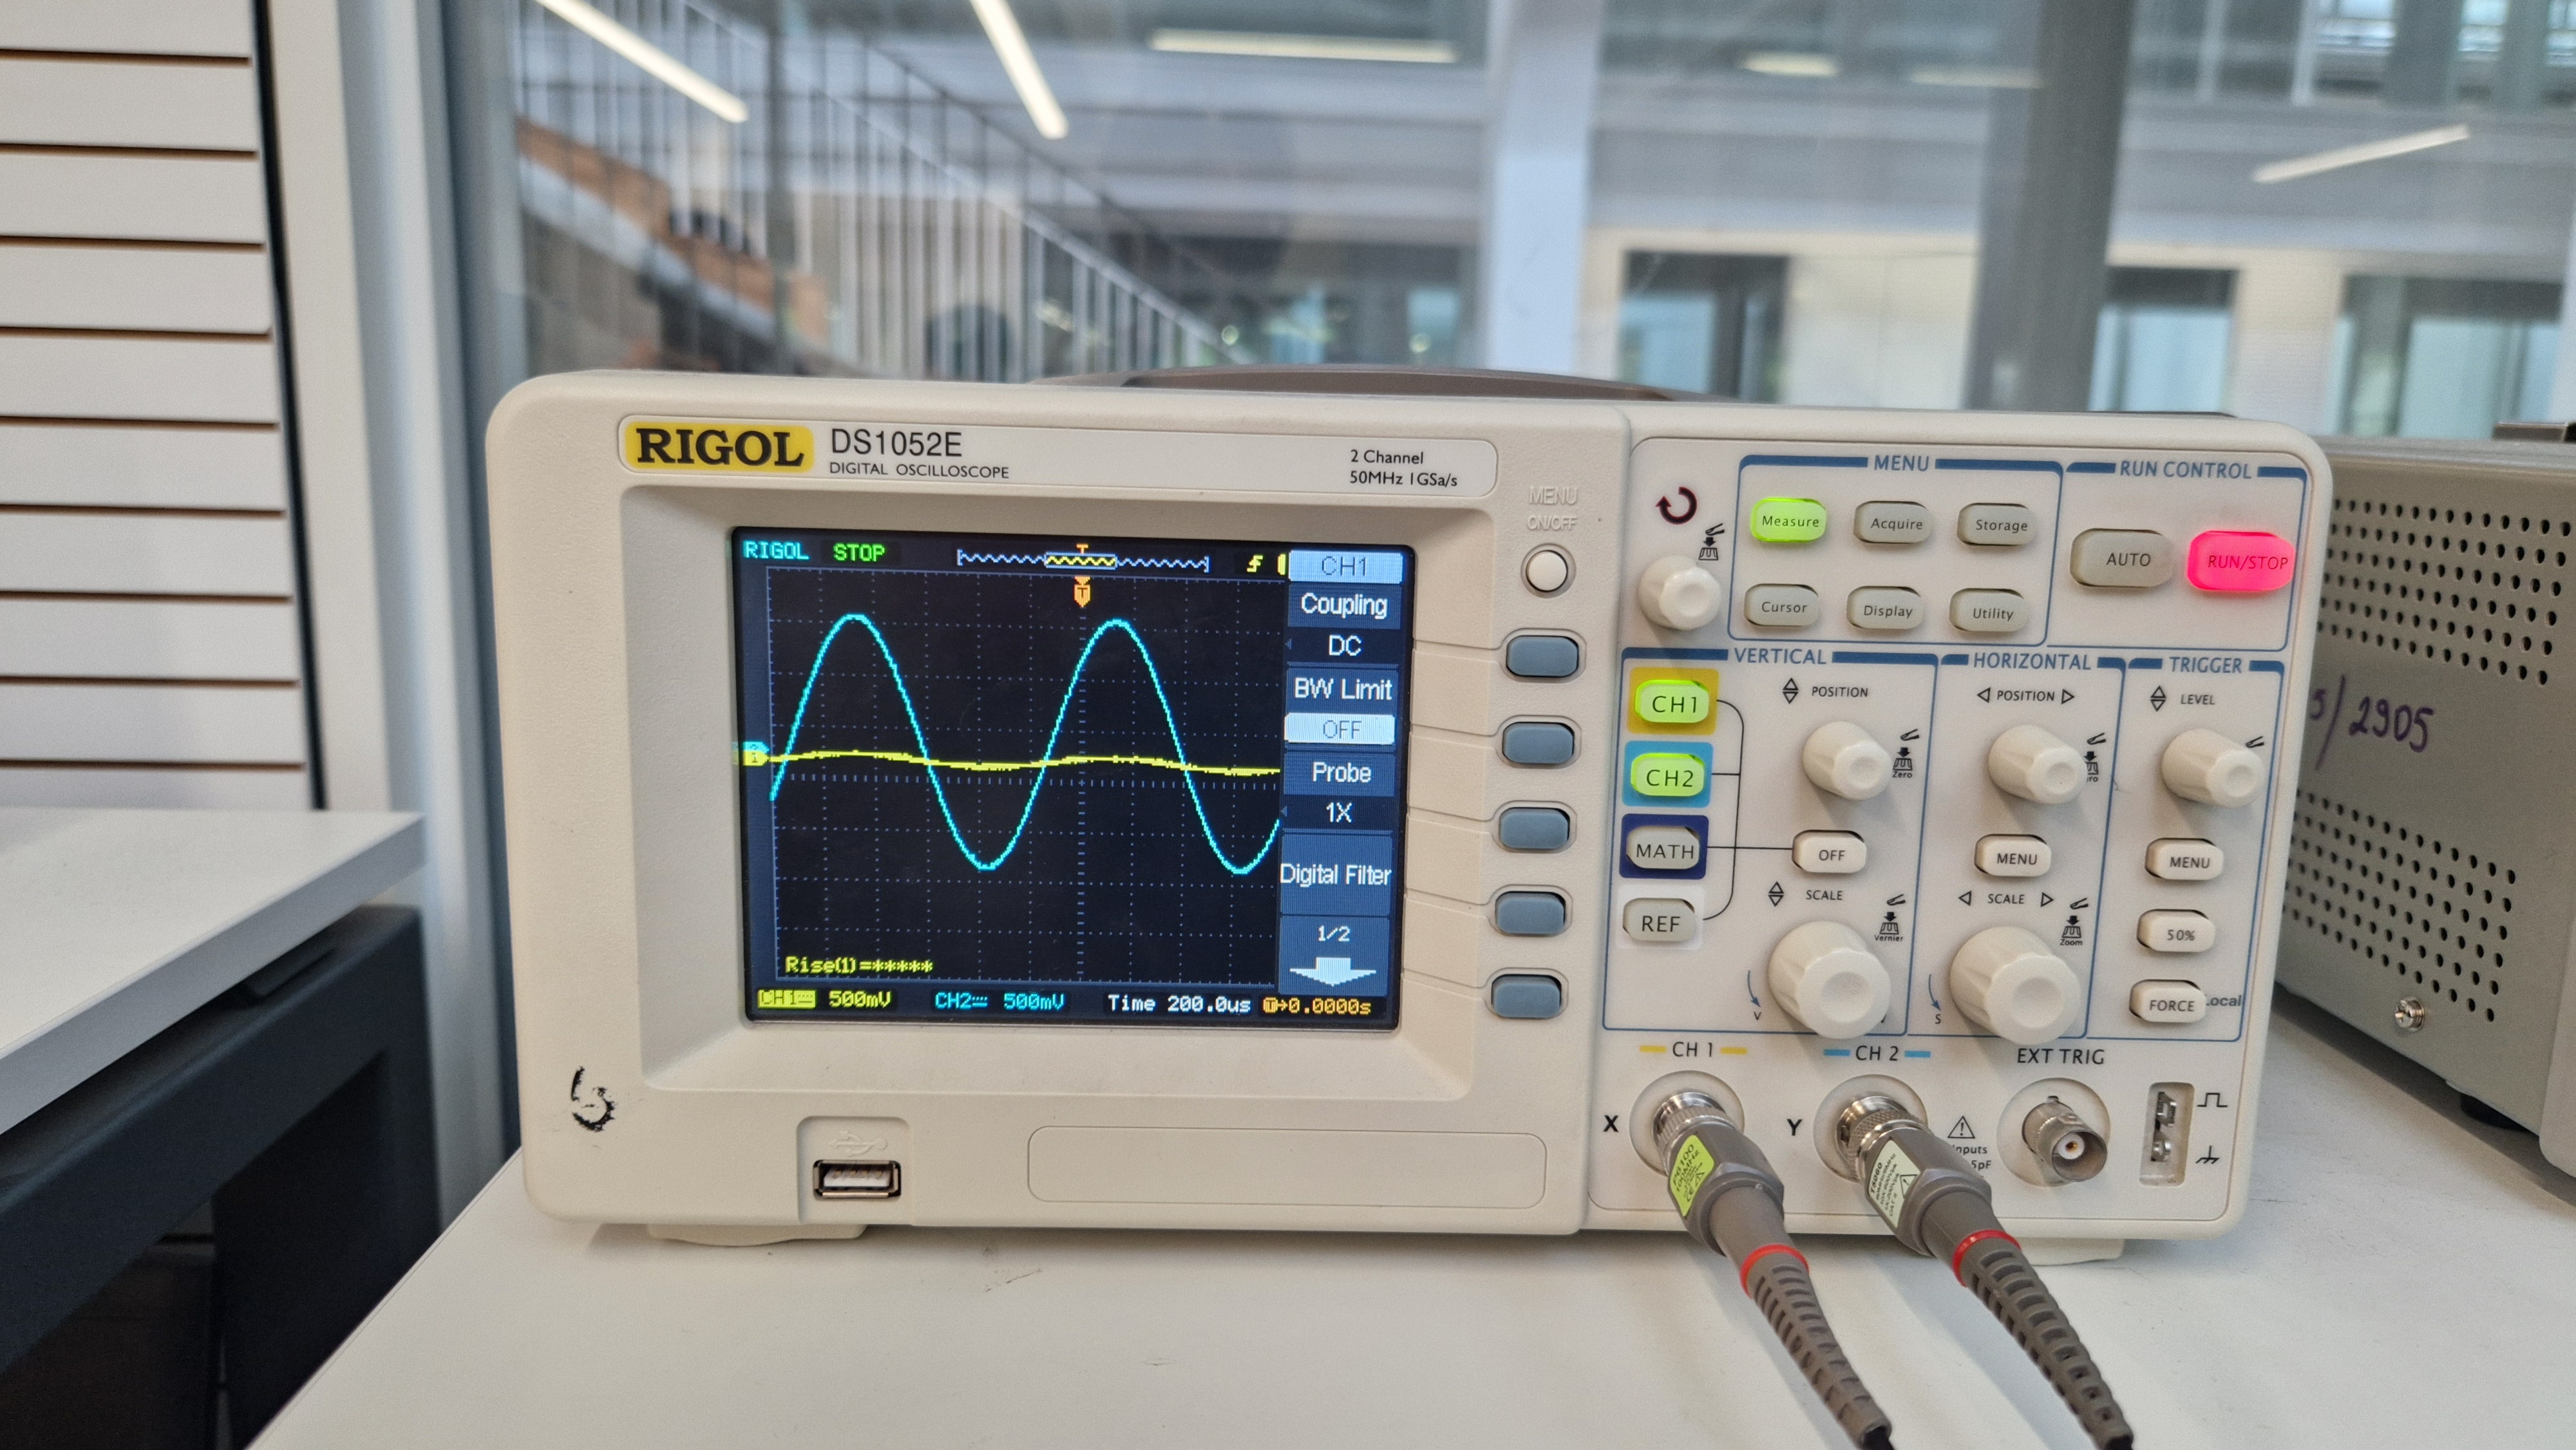
\includegraphics[width=0.6\textwidth]{assets/non-inverting-100m-output.jpg}
    \caption{Non-inverting @ 100mV}
    \label{fig:non-inverting-100m-output}
\end{figure}

Applying 100mV input to the non-inverting amplifier, the output is close to 2.3V as expected. The experiment result is shown in Figure \ref{fig:non-inverting-100m-output}. 

\newpage
\thispagestyle{plain}

\begin{figure}[h]
    \centering
    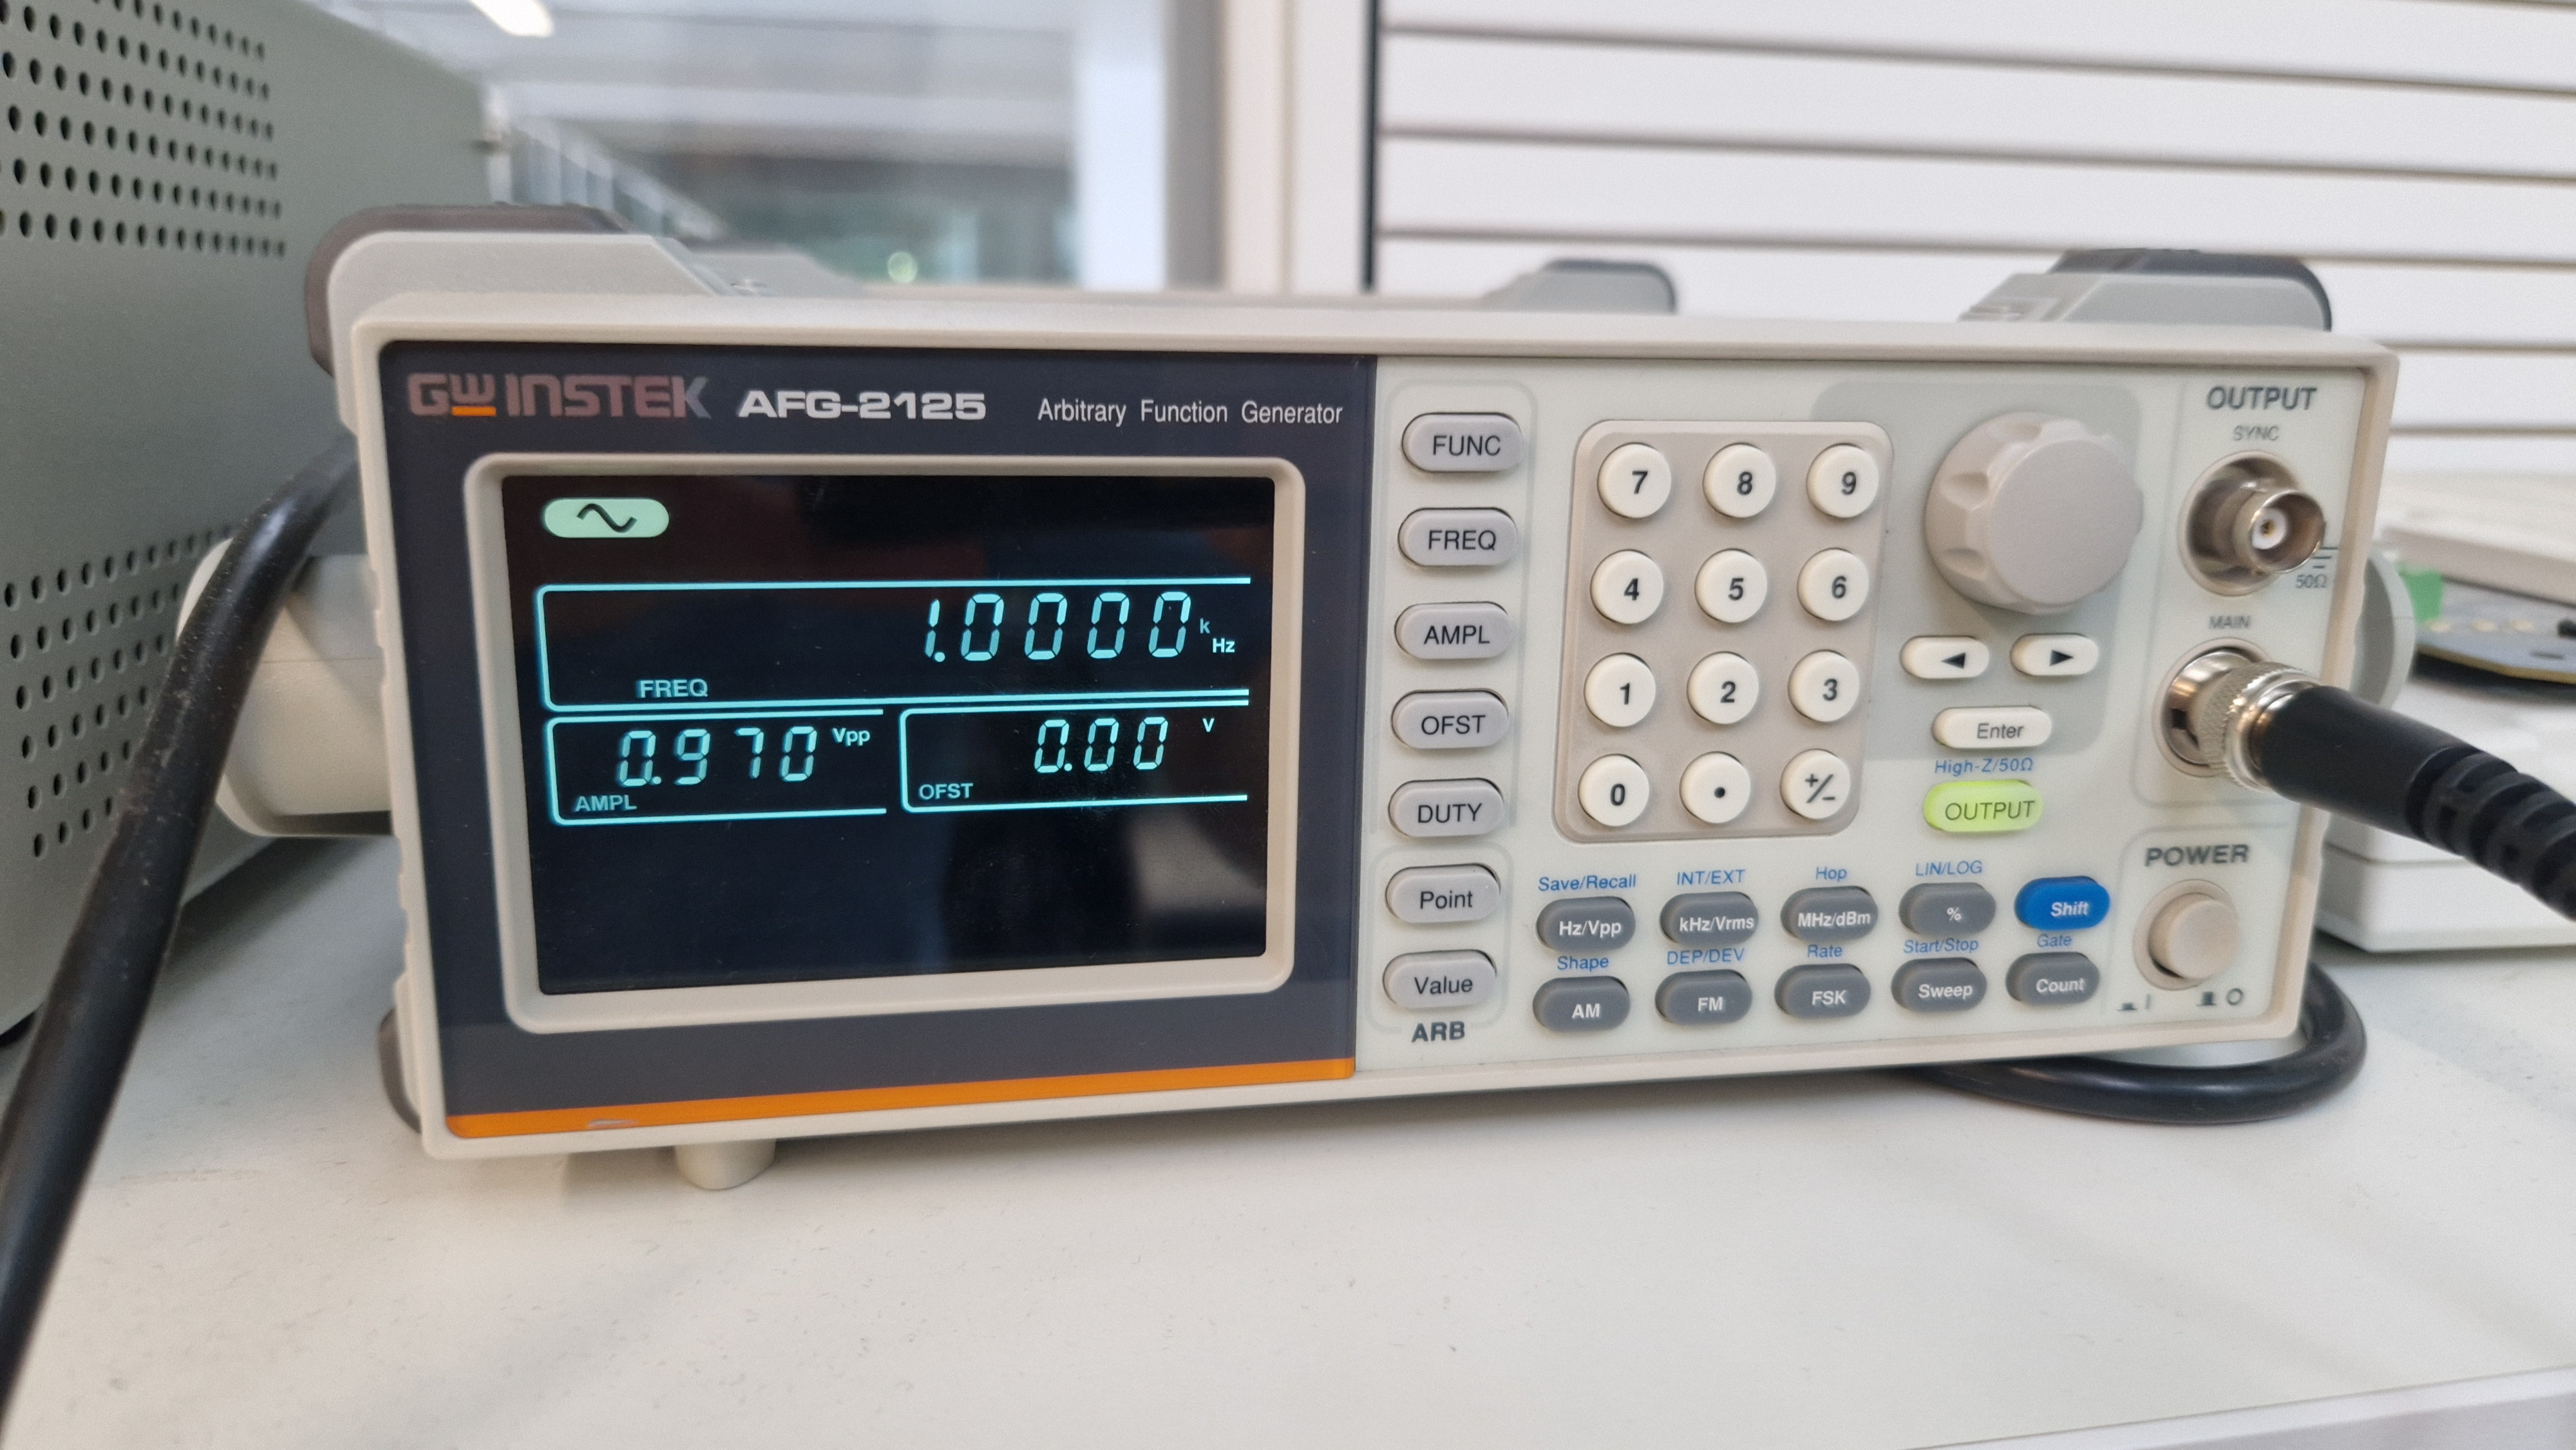
\includegraphics[width=0.6\textwidth]{assets/non-inverting-970m.jpg}
    \caption{Signal Generator @ 970mV}
    \label{fig:non-inverting-970m}
\end{figure}

\begin{figure}[h]
    \centering
    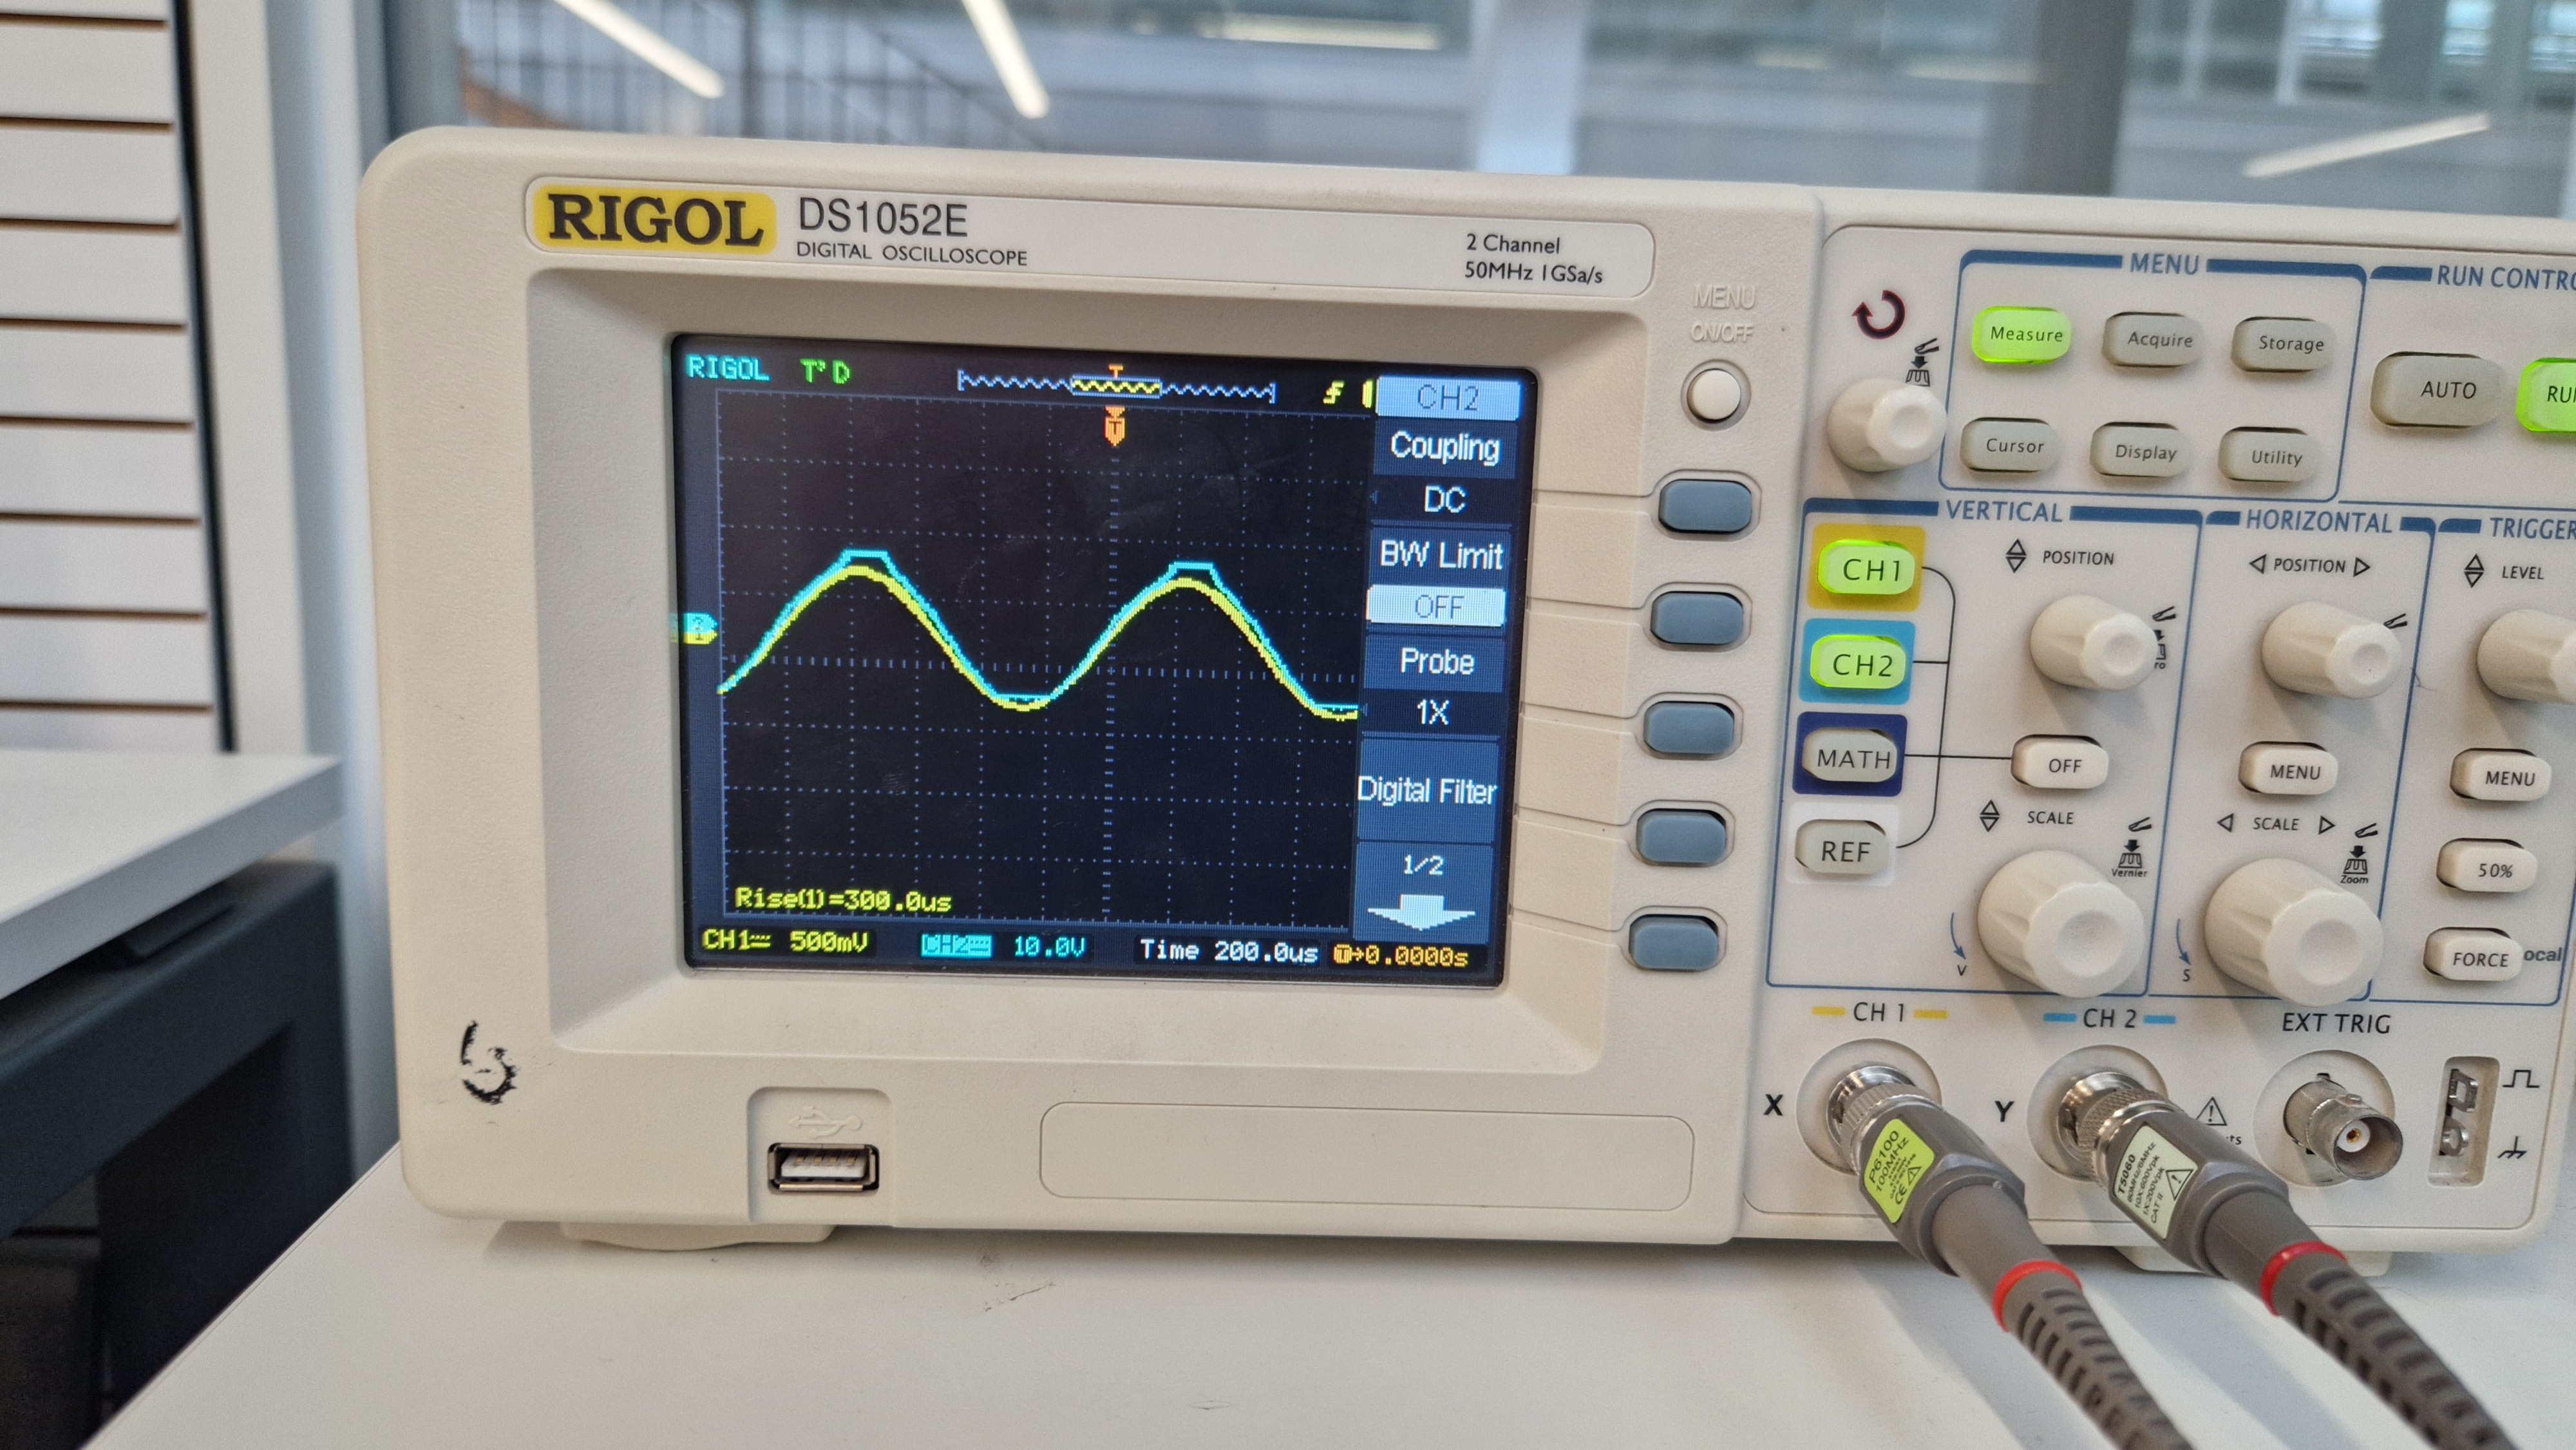
\includegraphics[width=0.6\textwidth]{assets/non-inverting-970m-output.jpg}
    \caption{Non-inverting @ 970mV}
    \label{fig:non-inverting-970m-output}
\end{figure}

Applying 970mV input to the non-inverting amplifier, the output should be 13.7V but it is limited to 12V due to the power supply as seen in Figure \ref{fig:non-inverting-970m-output}.

\newpage
\thispagestyle{plain}

\begin{figure}[h]
    \centering
    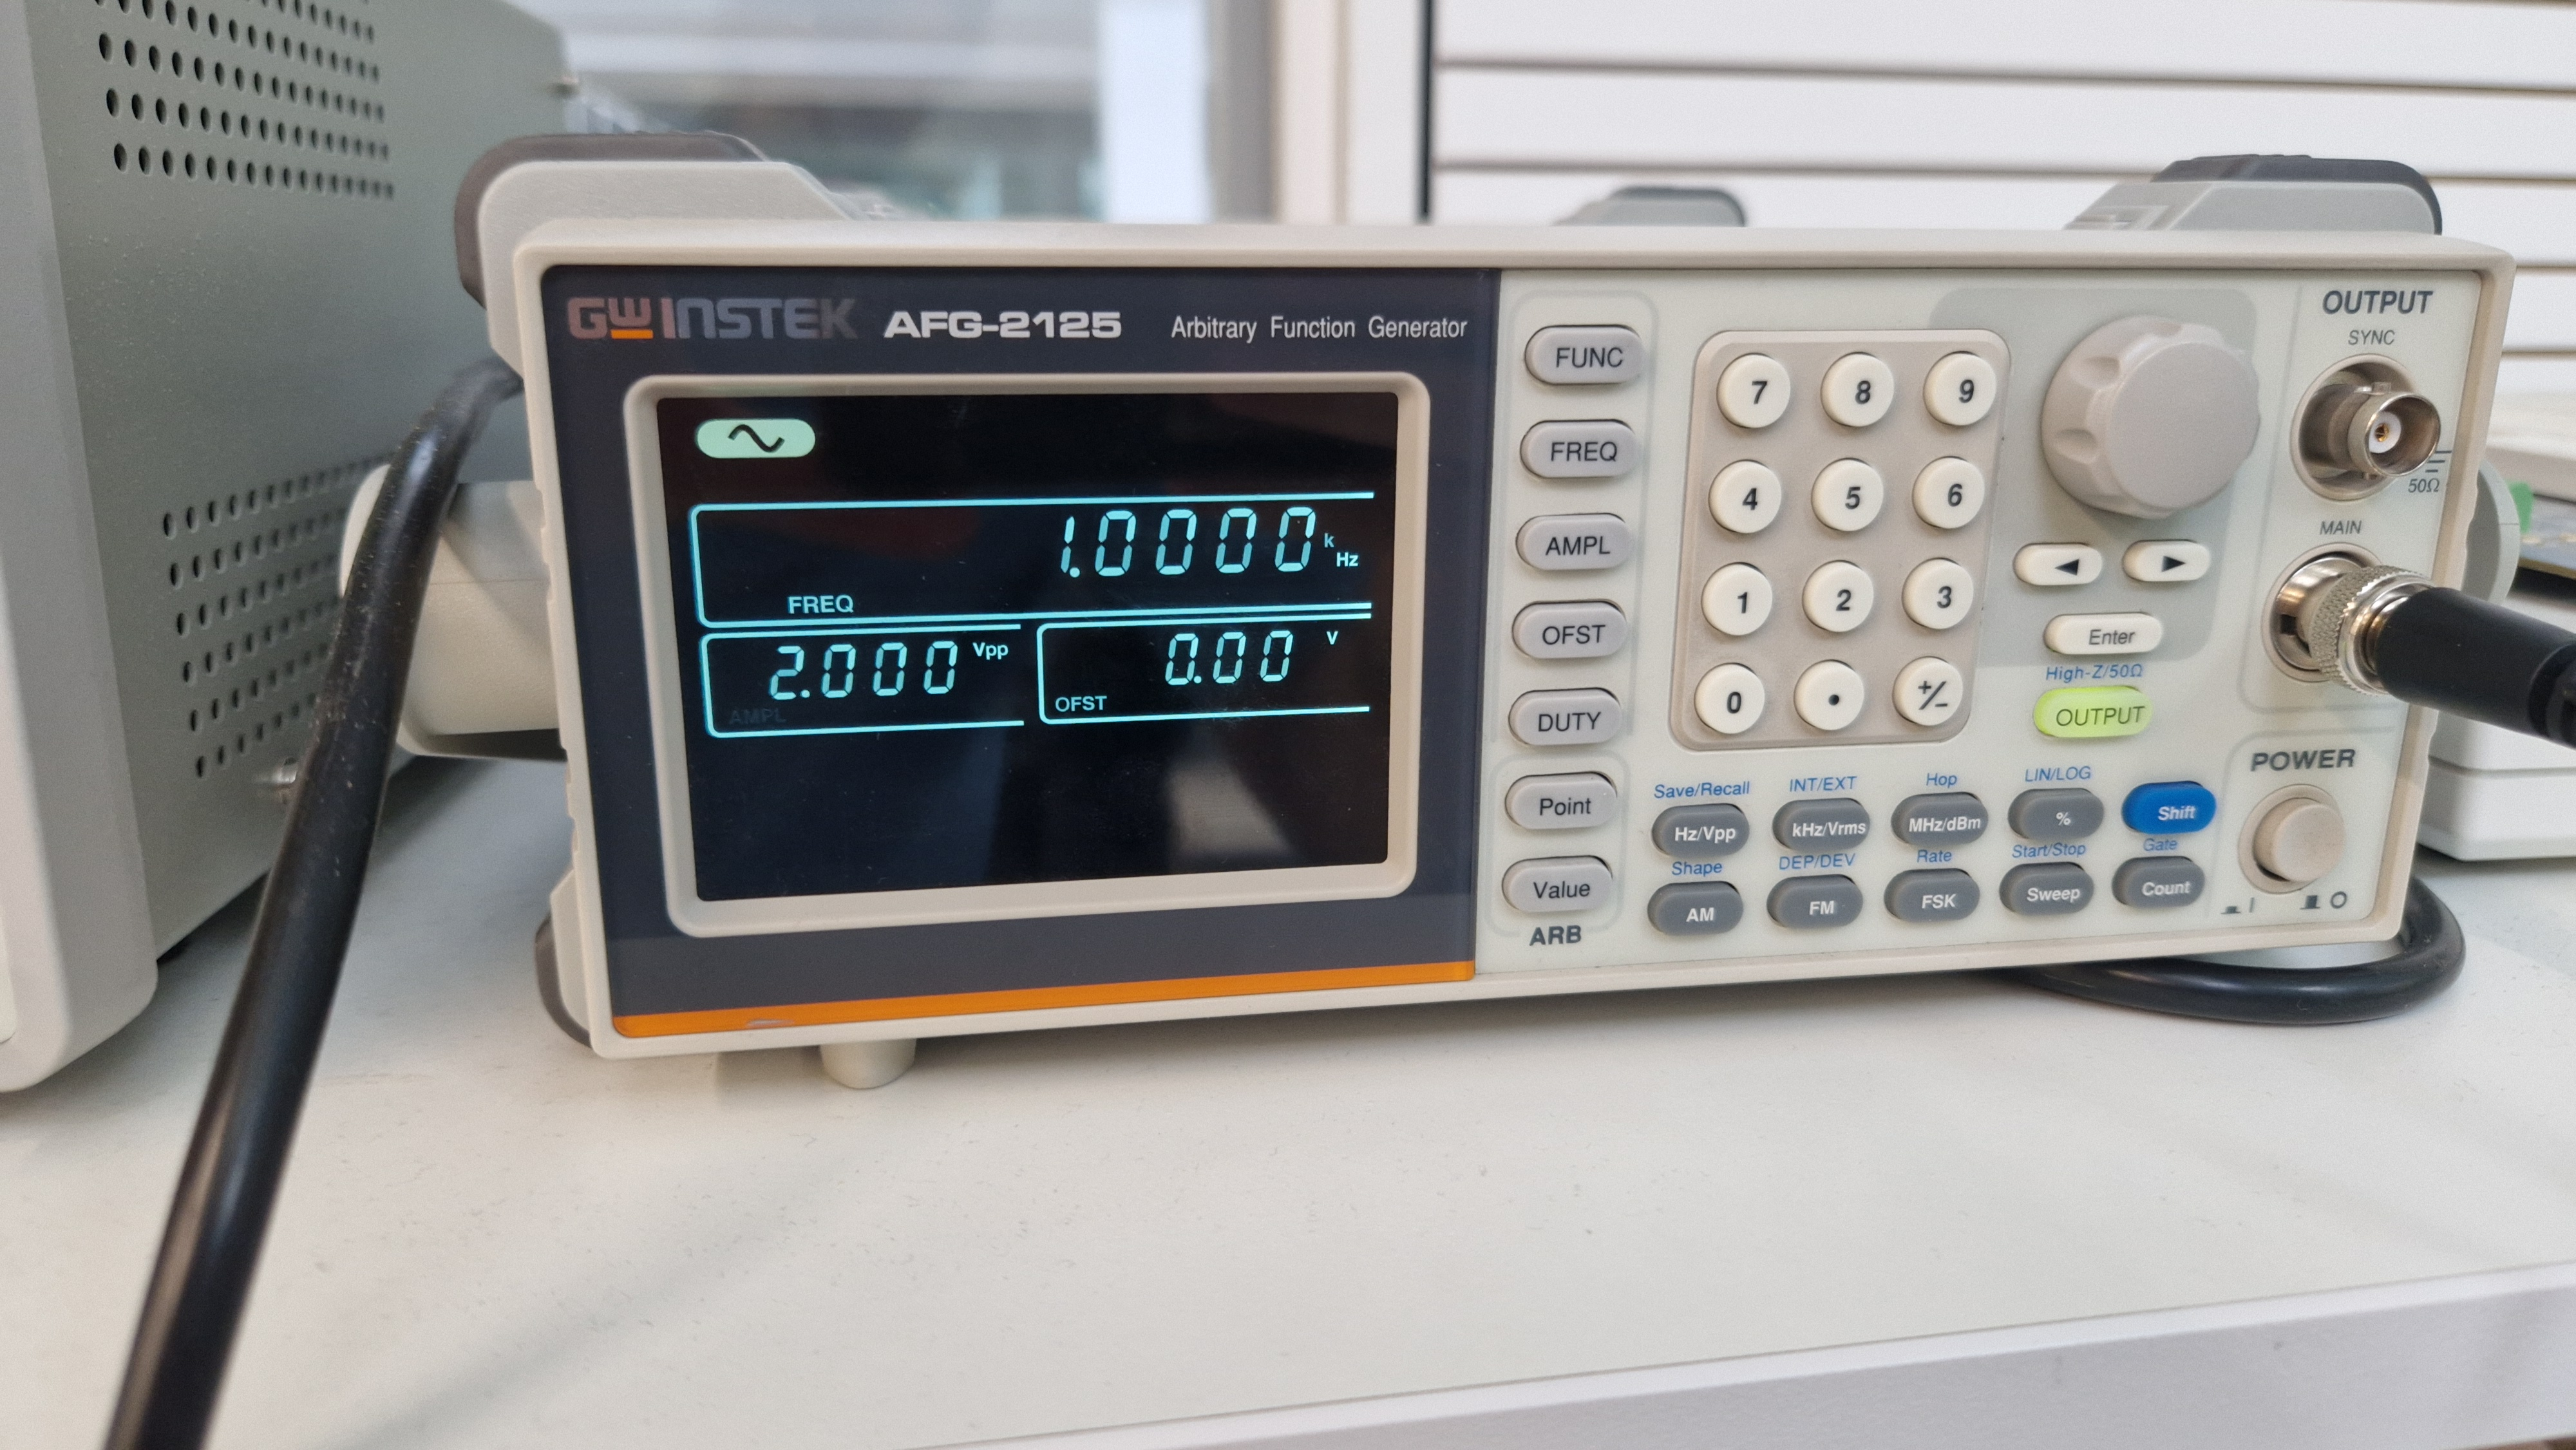
\includegraphics[width=0.6\textwidth]{assets/non-inverting-2.jpg}
    \caption{Signal Generator @ 2V}
    \label{fig:non-inverting-2}
\end{figure}

\begin{figure}[h]
    \centering
    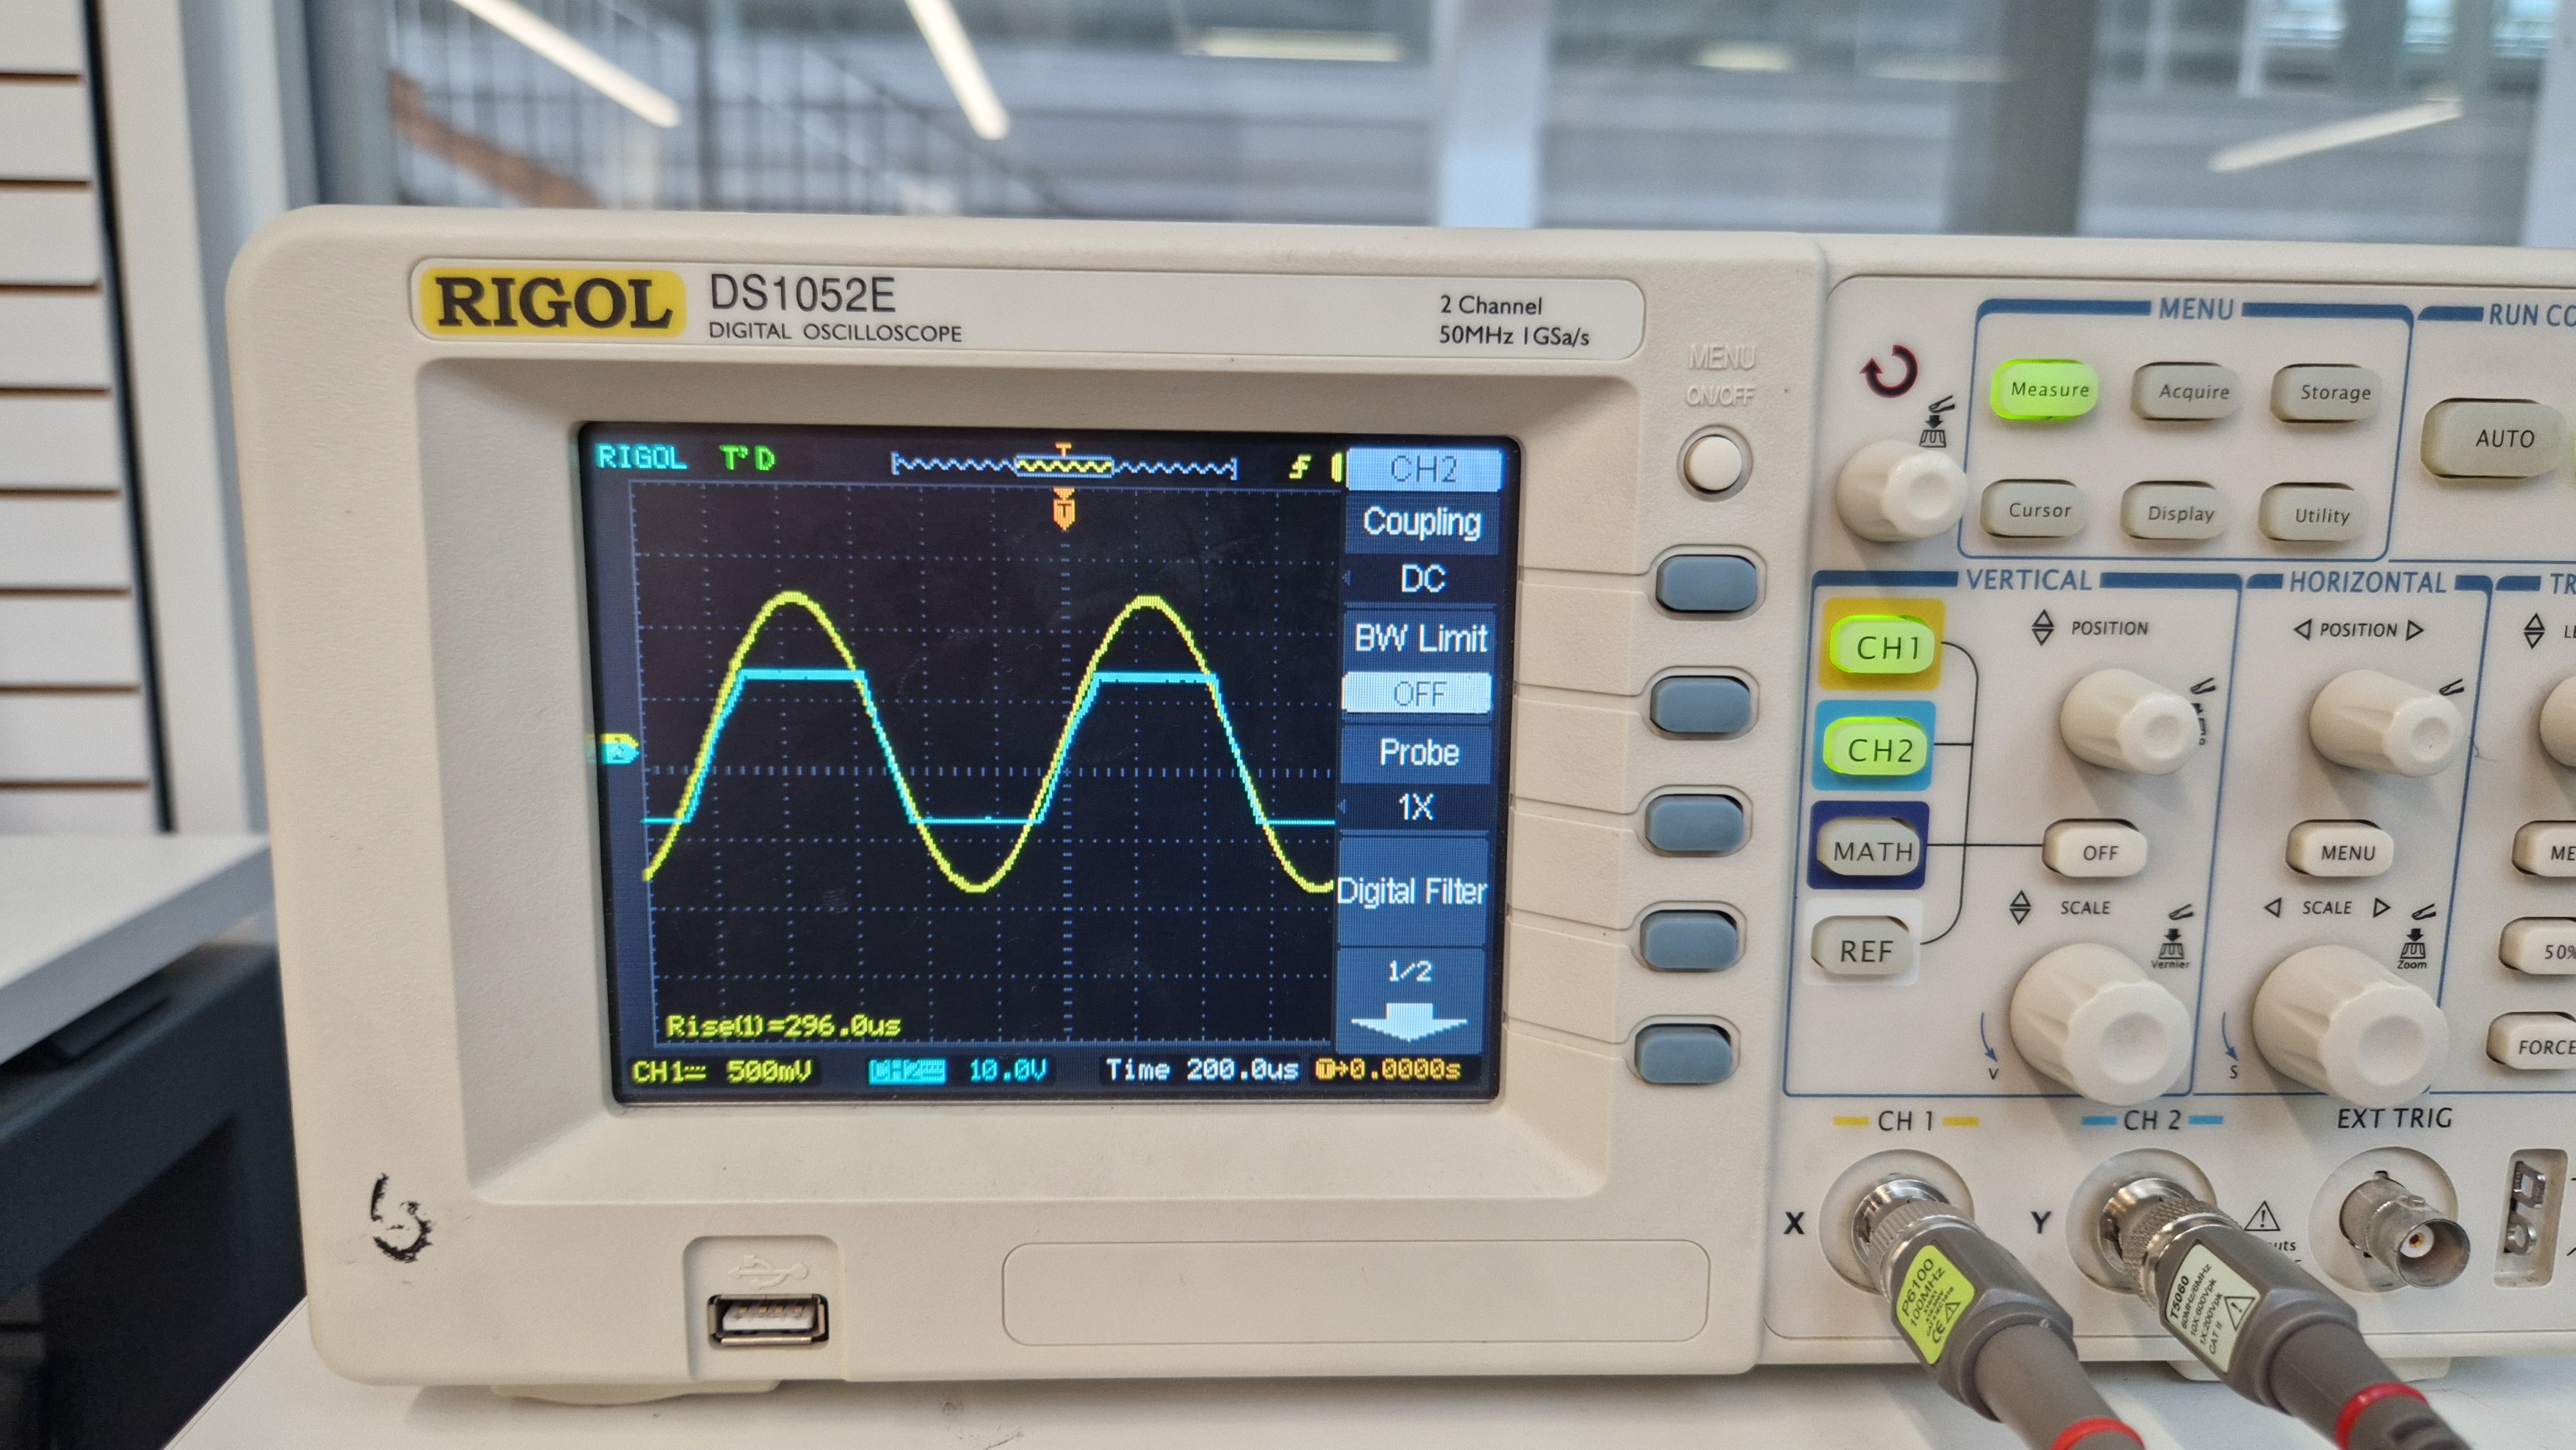
\includegraphics[width=0.6\textwidth]{assets/non-inverting-2-output.jpg}
    \caption{Non-inverting @ 2V}
    \label{fig:non-inverting-2-output}
\end{figure}

Applying 1V input to the non-inverting amplifier, the output should be 23V but it is limited to 12V due to the power supply as it is \textbf{more visible} in Figure \ref{fig:non-inverting-2-output}.

\newpage
\thispagestyle{plain}

\subsection{Inverting Amplifier}

\begin{figure}[h]
    \centering
    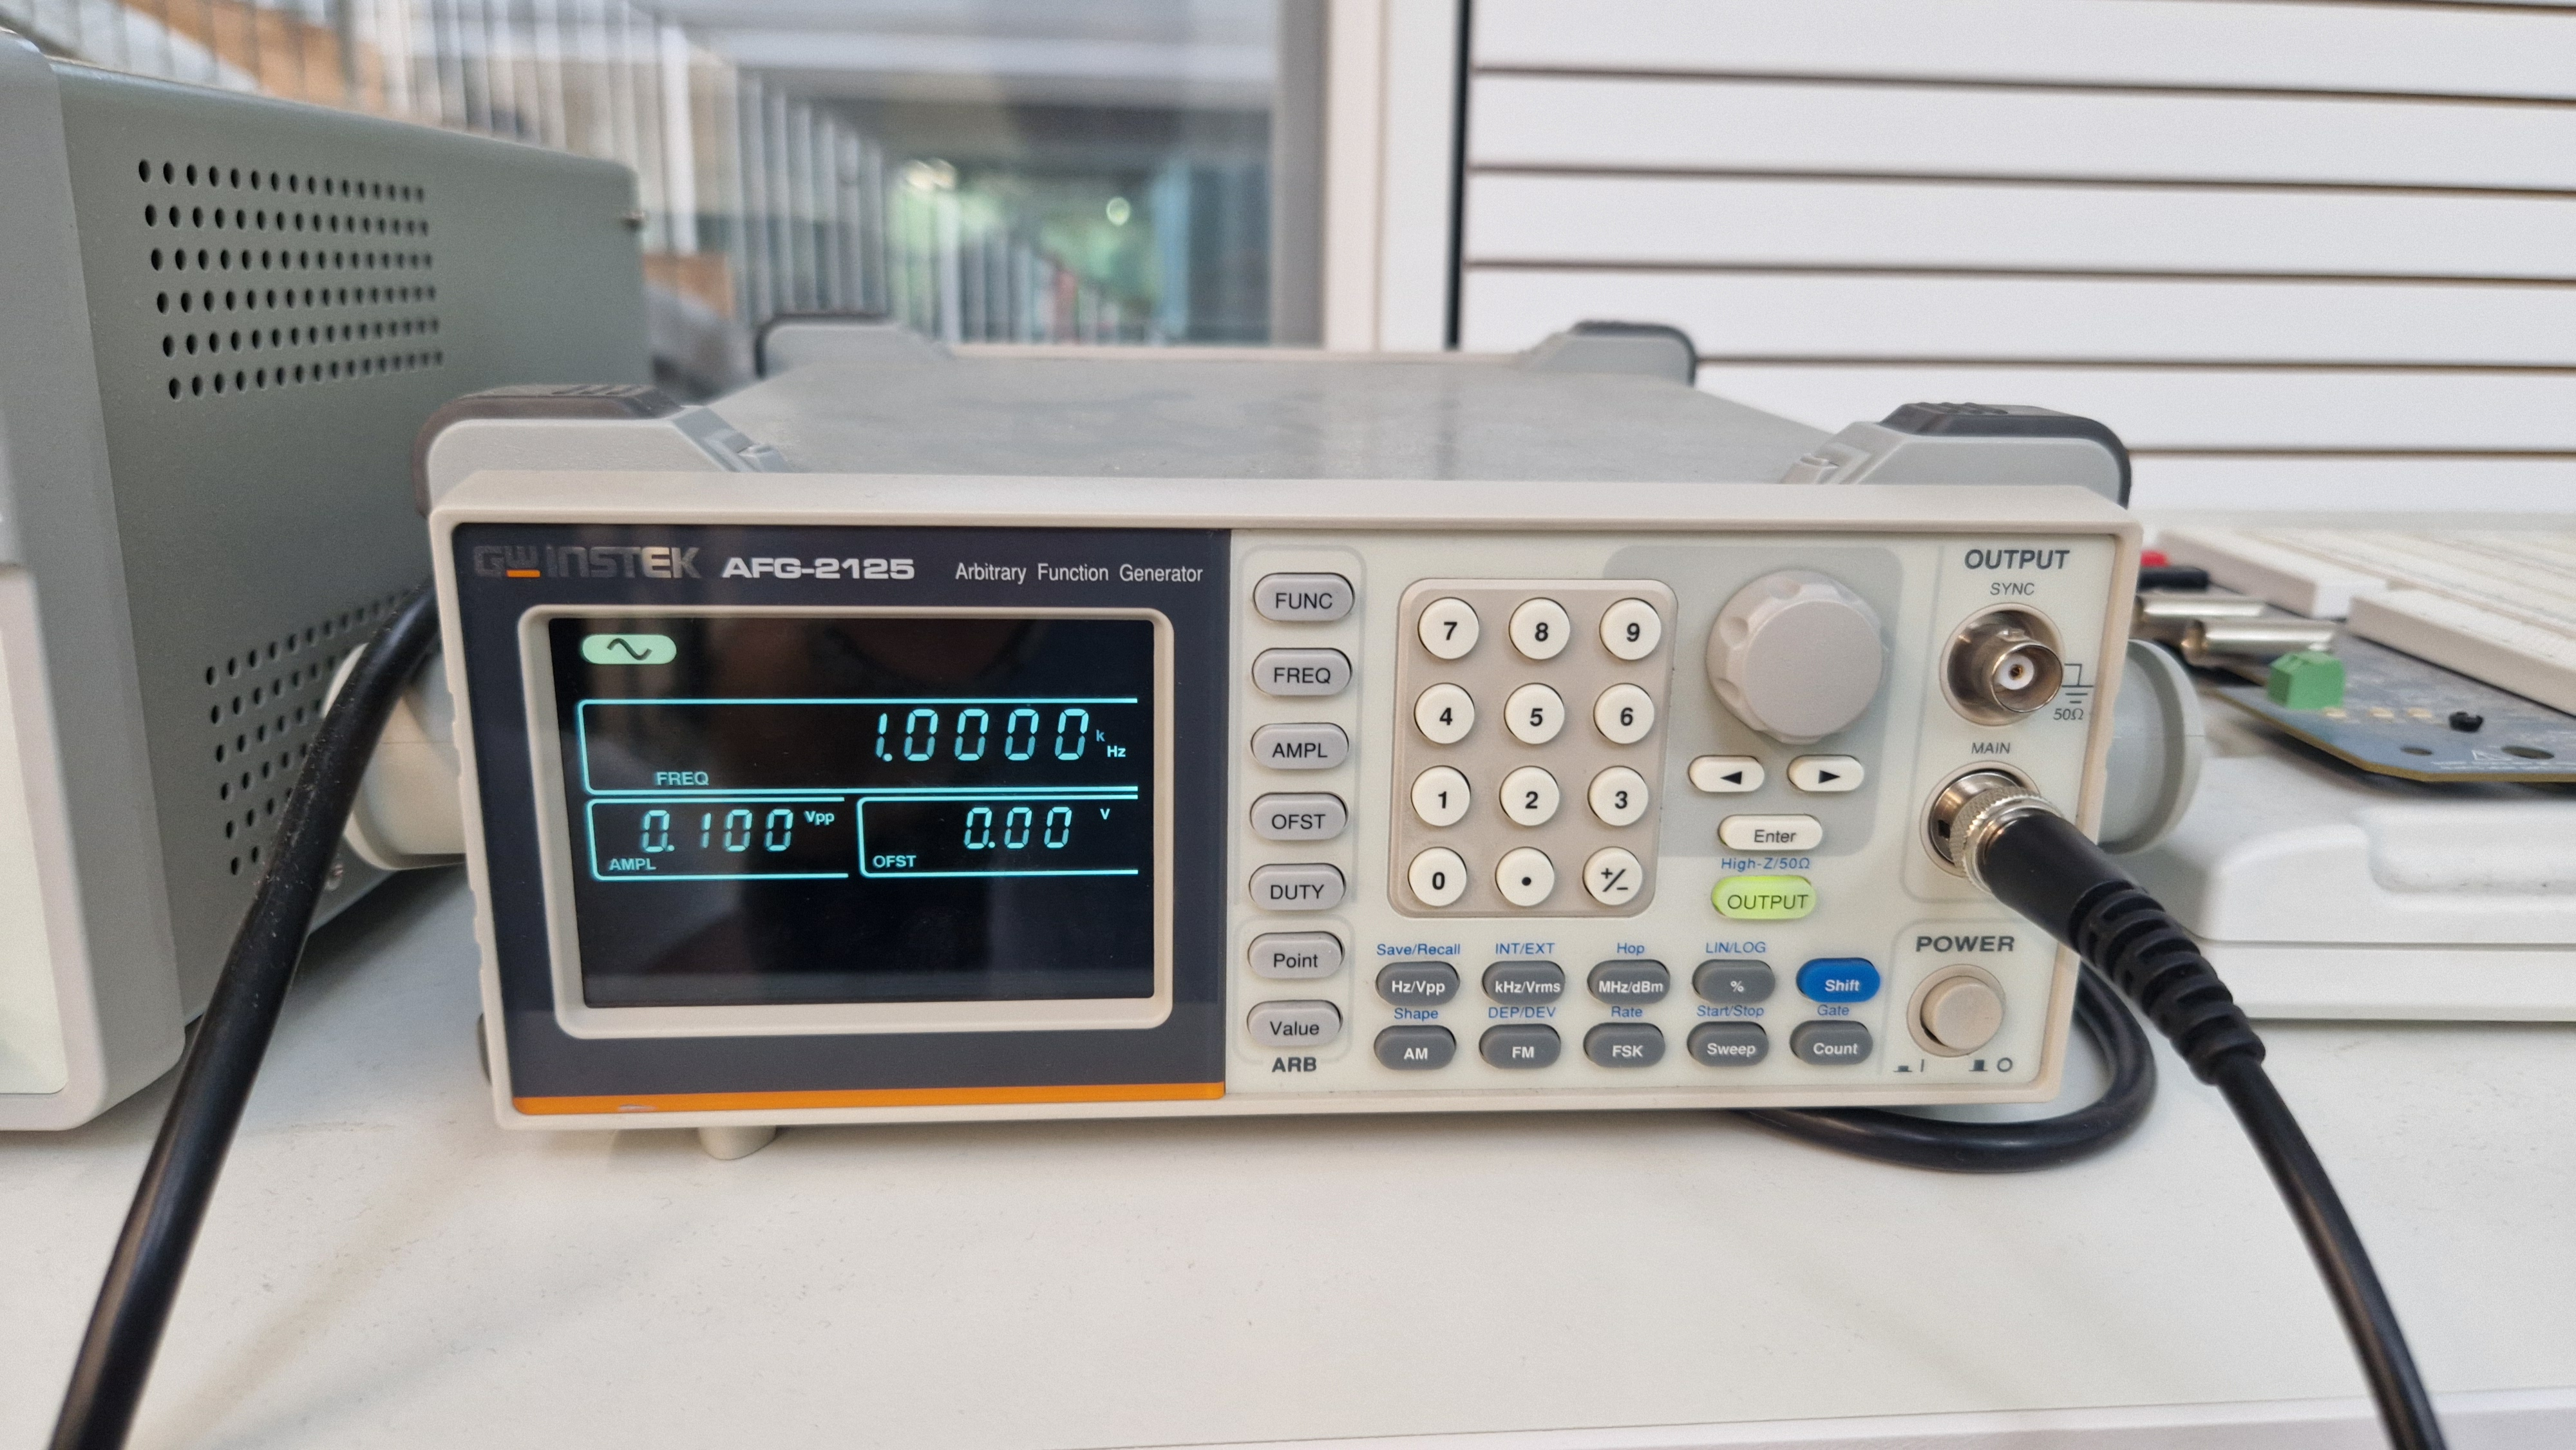
\includegraphics[width=0.6\textwidth]{assets/inverting-100.jpg}
    \caption{Signal Generator @ 100mV}
    \label{fig:inverting-100m}
\end{figure}

\begin{figure}[h]
    \centering
    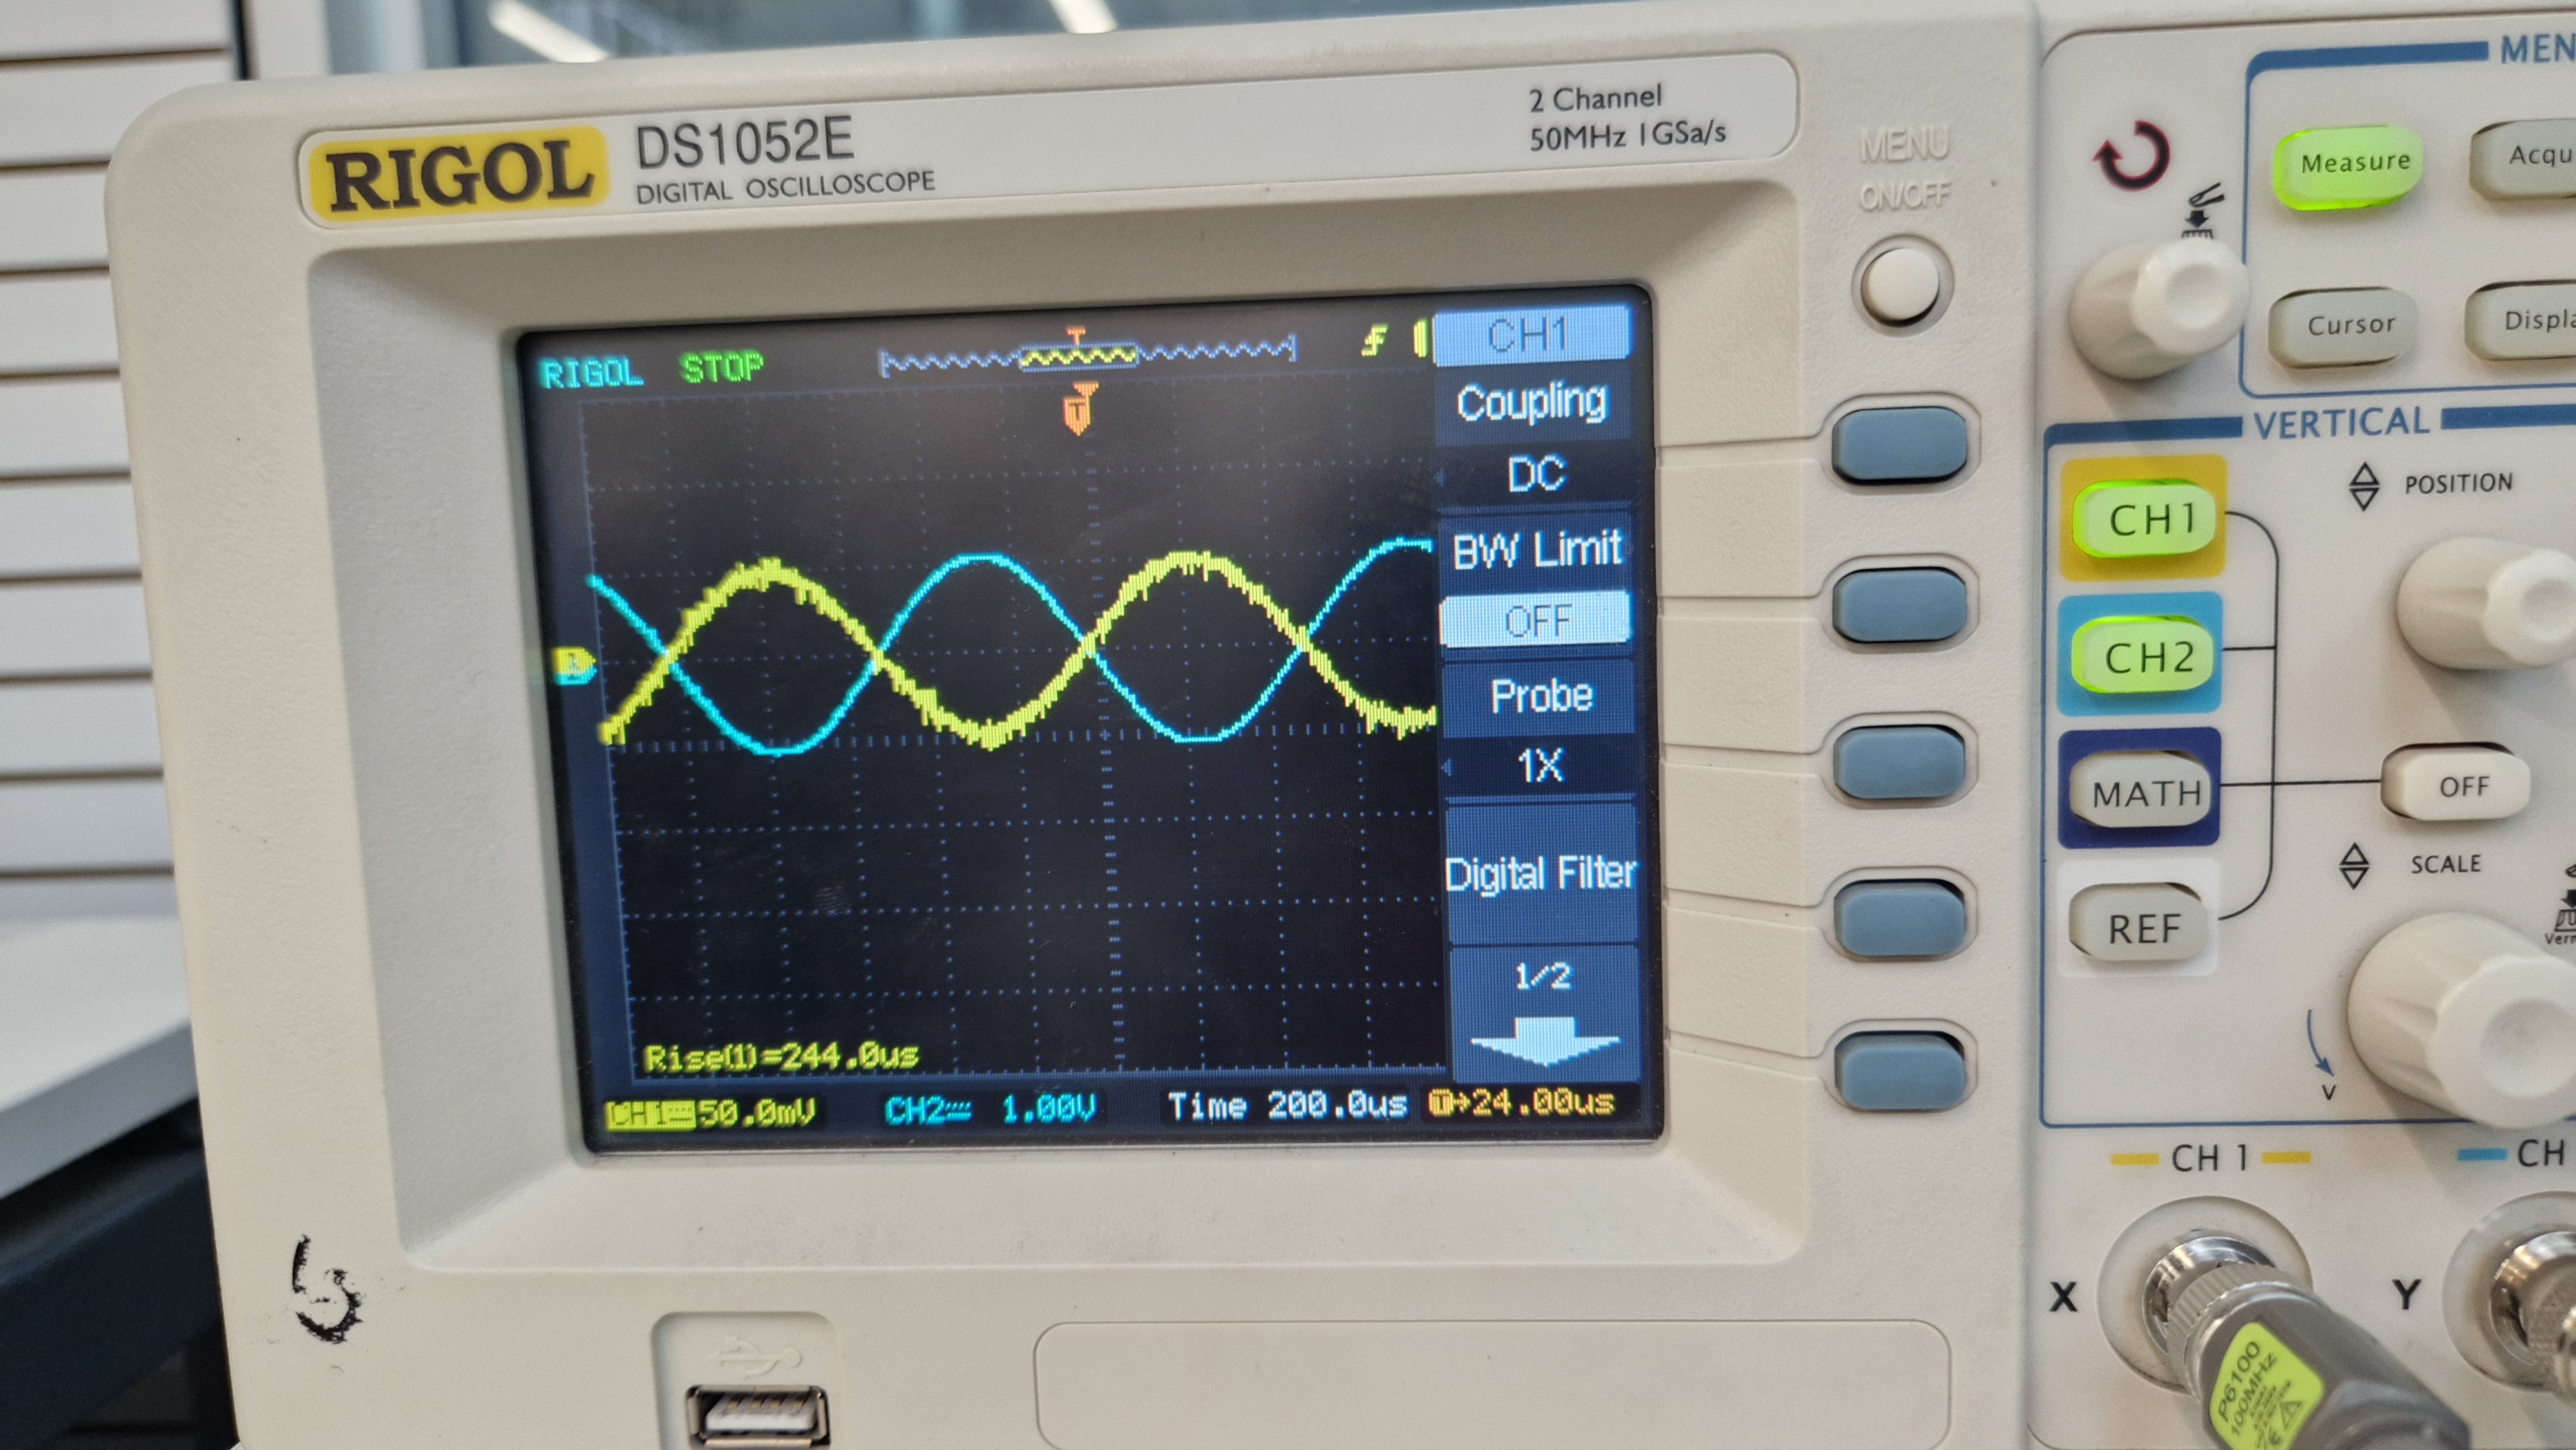
\includegraphics[width=0.6\textwidth]{assets/inverting-100-output.jpg}
    \caption{Inverting @ 100mV}
    \label{fig:inverting-100m-output}
\end{figure}

Applying 100mV input to the inverting amplifier, the output is close to -2.2V as expected. The experiment result is shown in Figure \ref{fig:inverting-100m-output}.

\newpage
\thispagestyle{plain}

\begin{figure}[h]
    \centering
    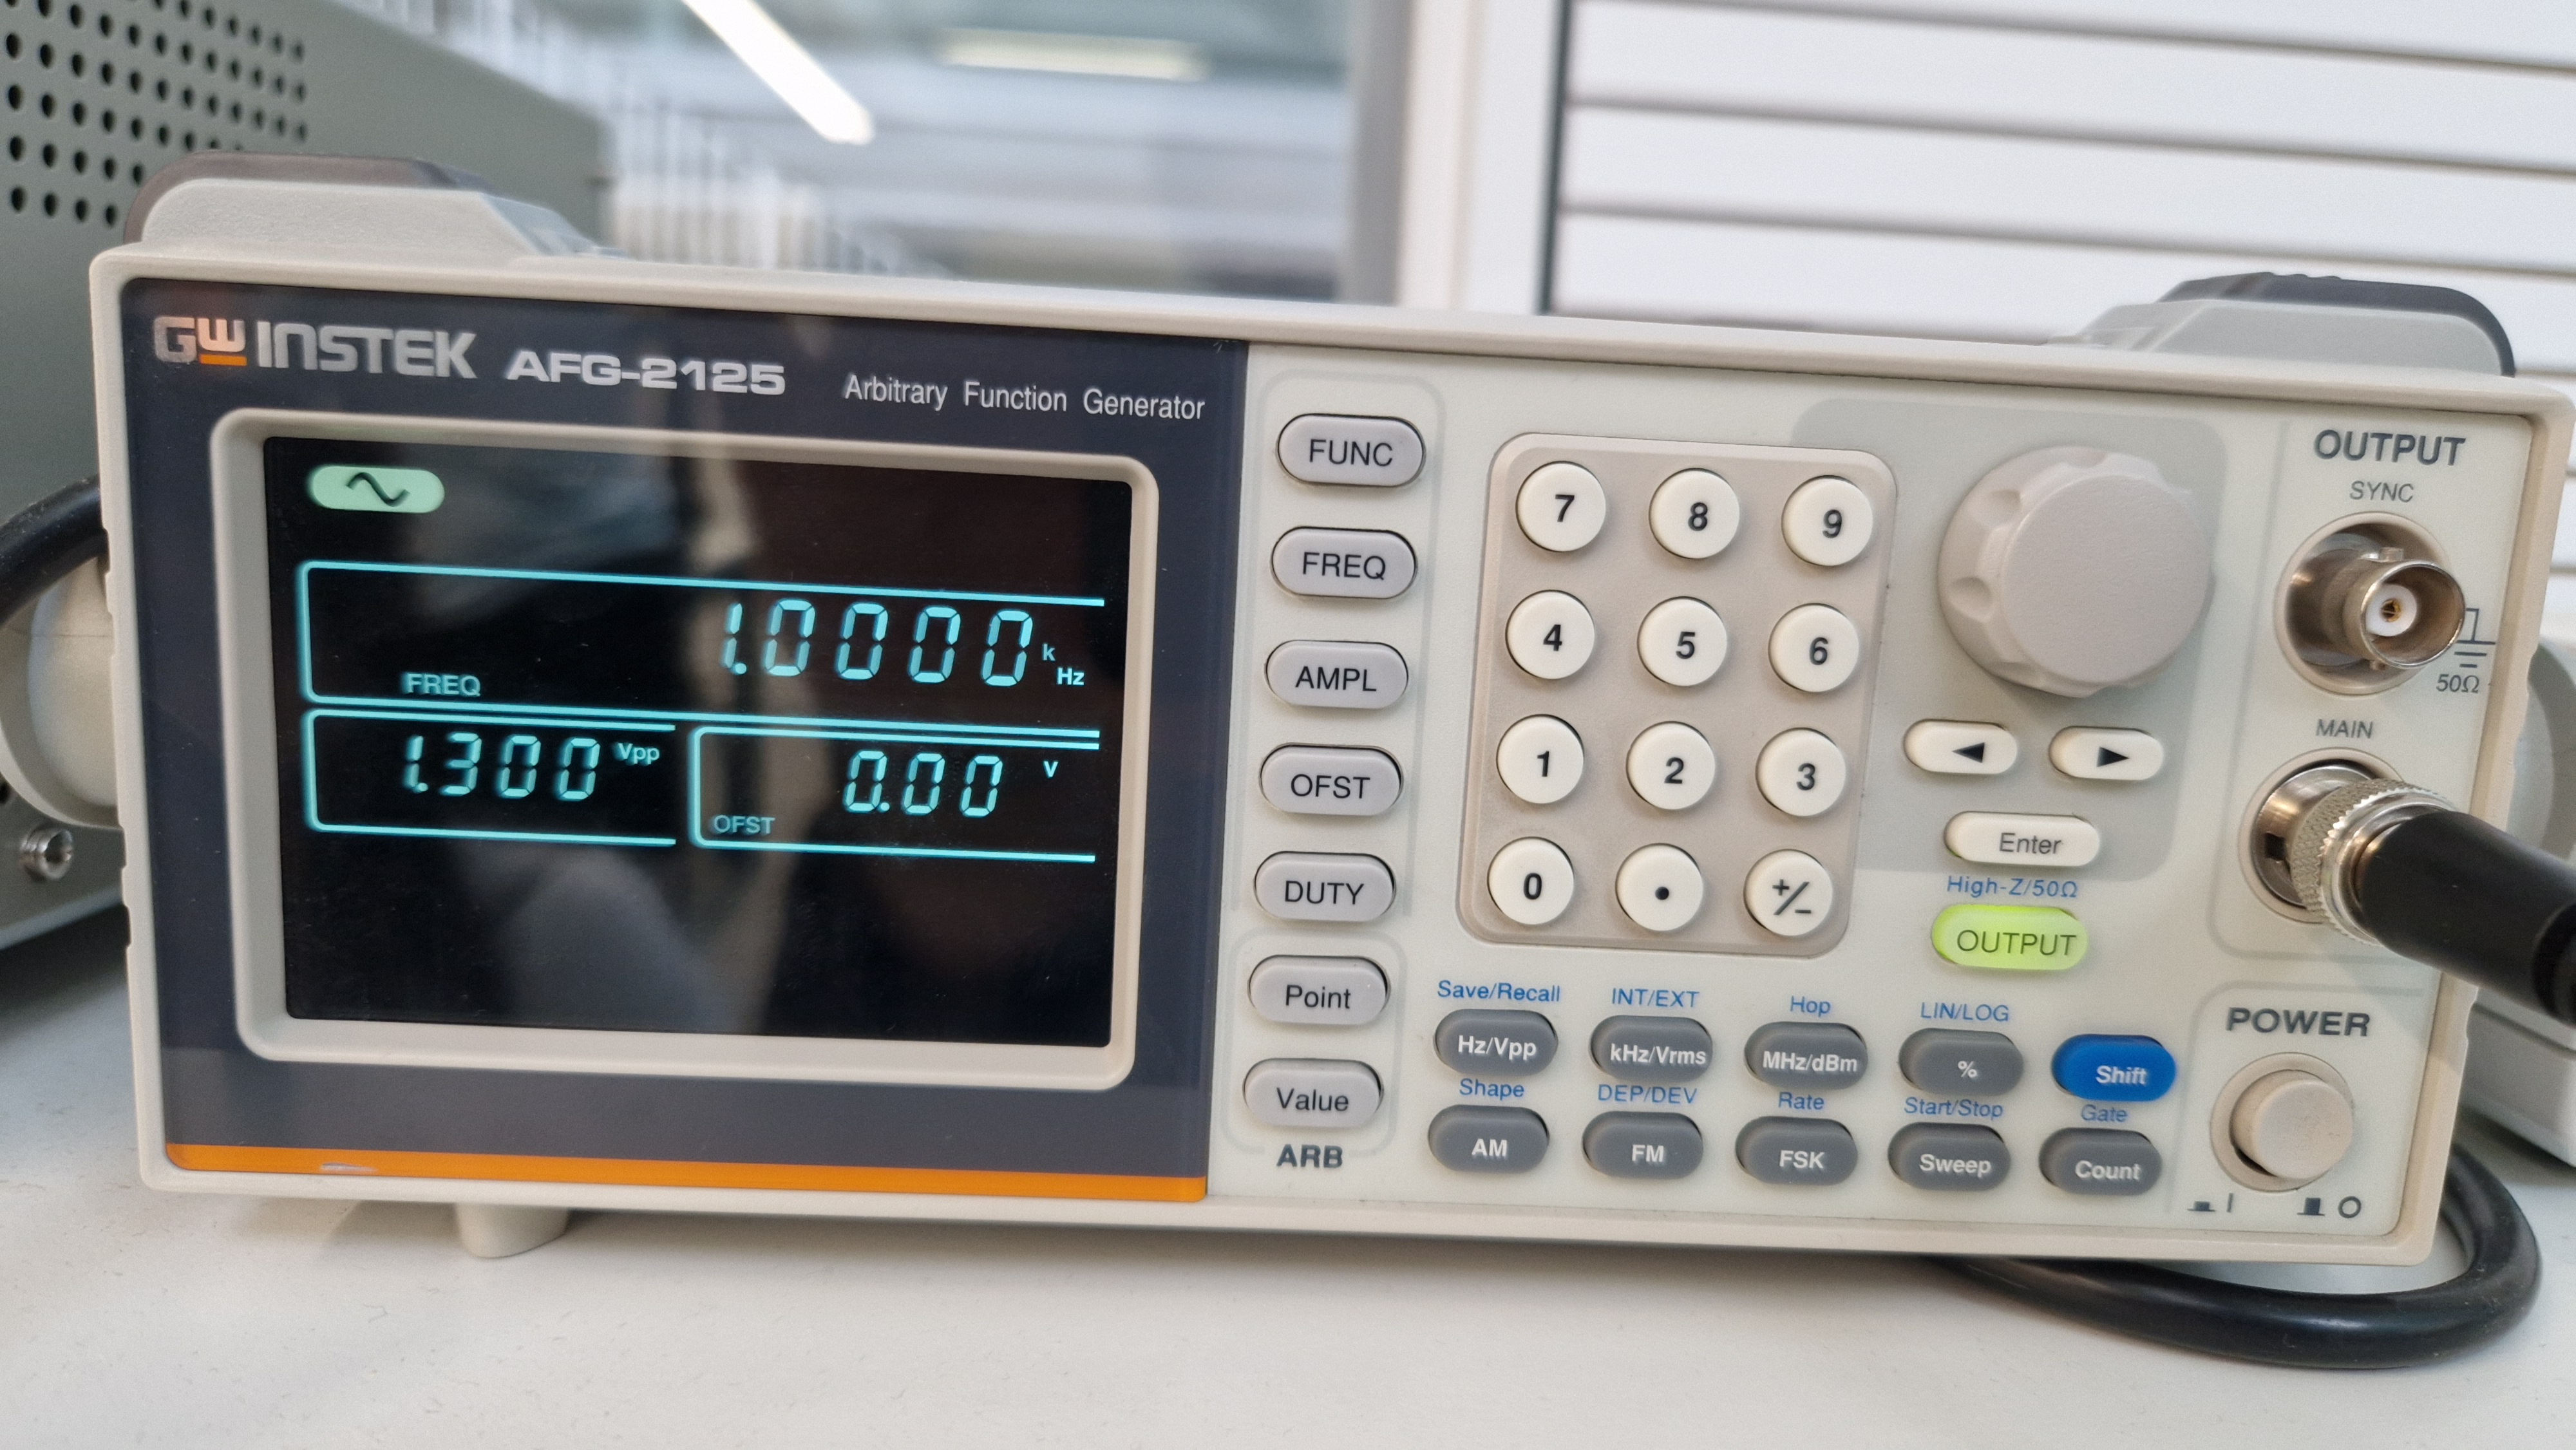
\includegraphics[width=0.6\textwidth]{assets/inverting-1.3.jpg}
    \caption{Signal Generator @ 1.3V}
    \label{fig:inverting-1.3}
\end{figure}

\begin{figure}[h]
    \centering
    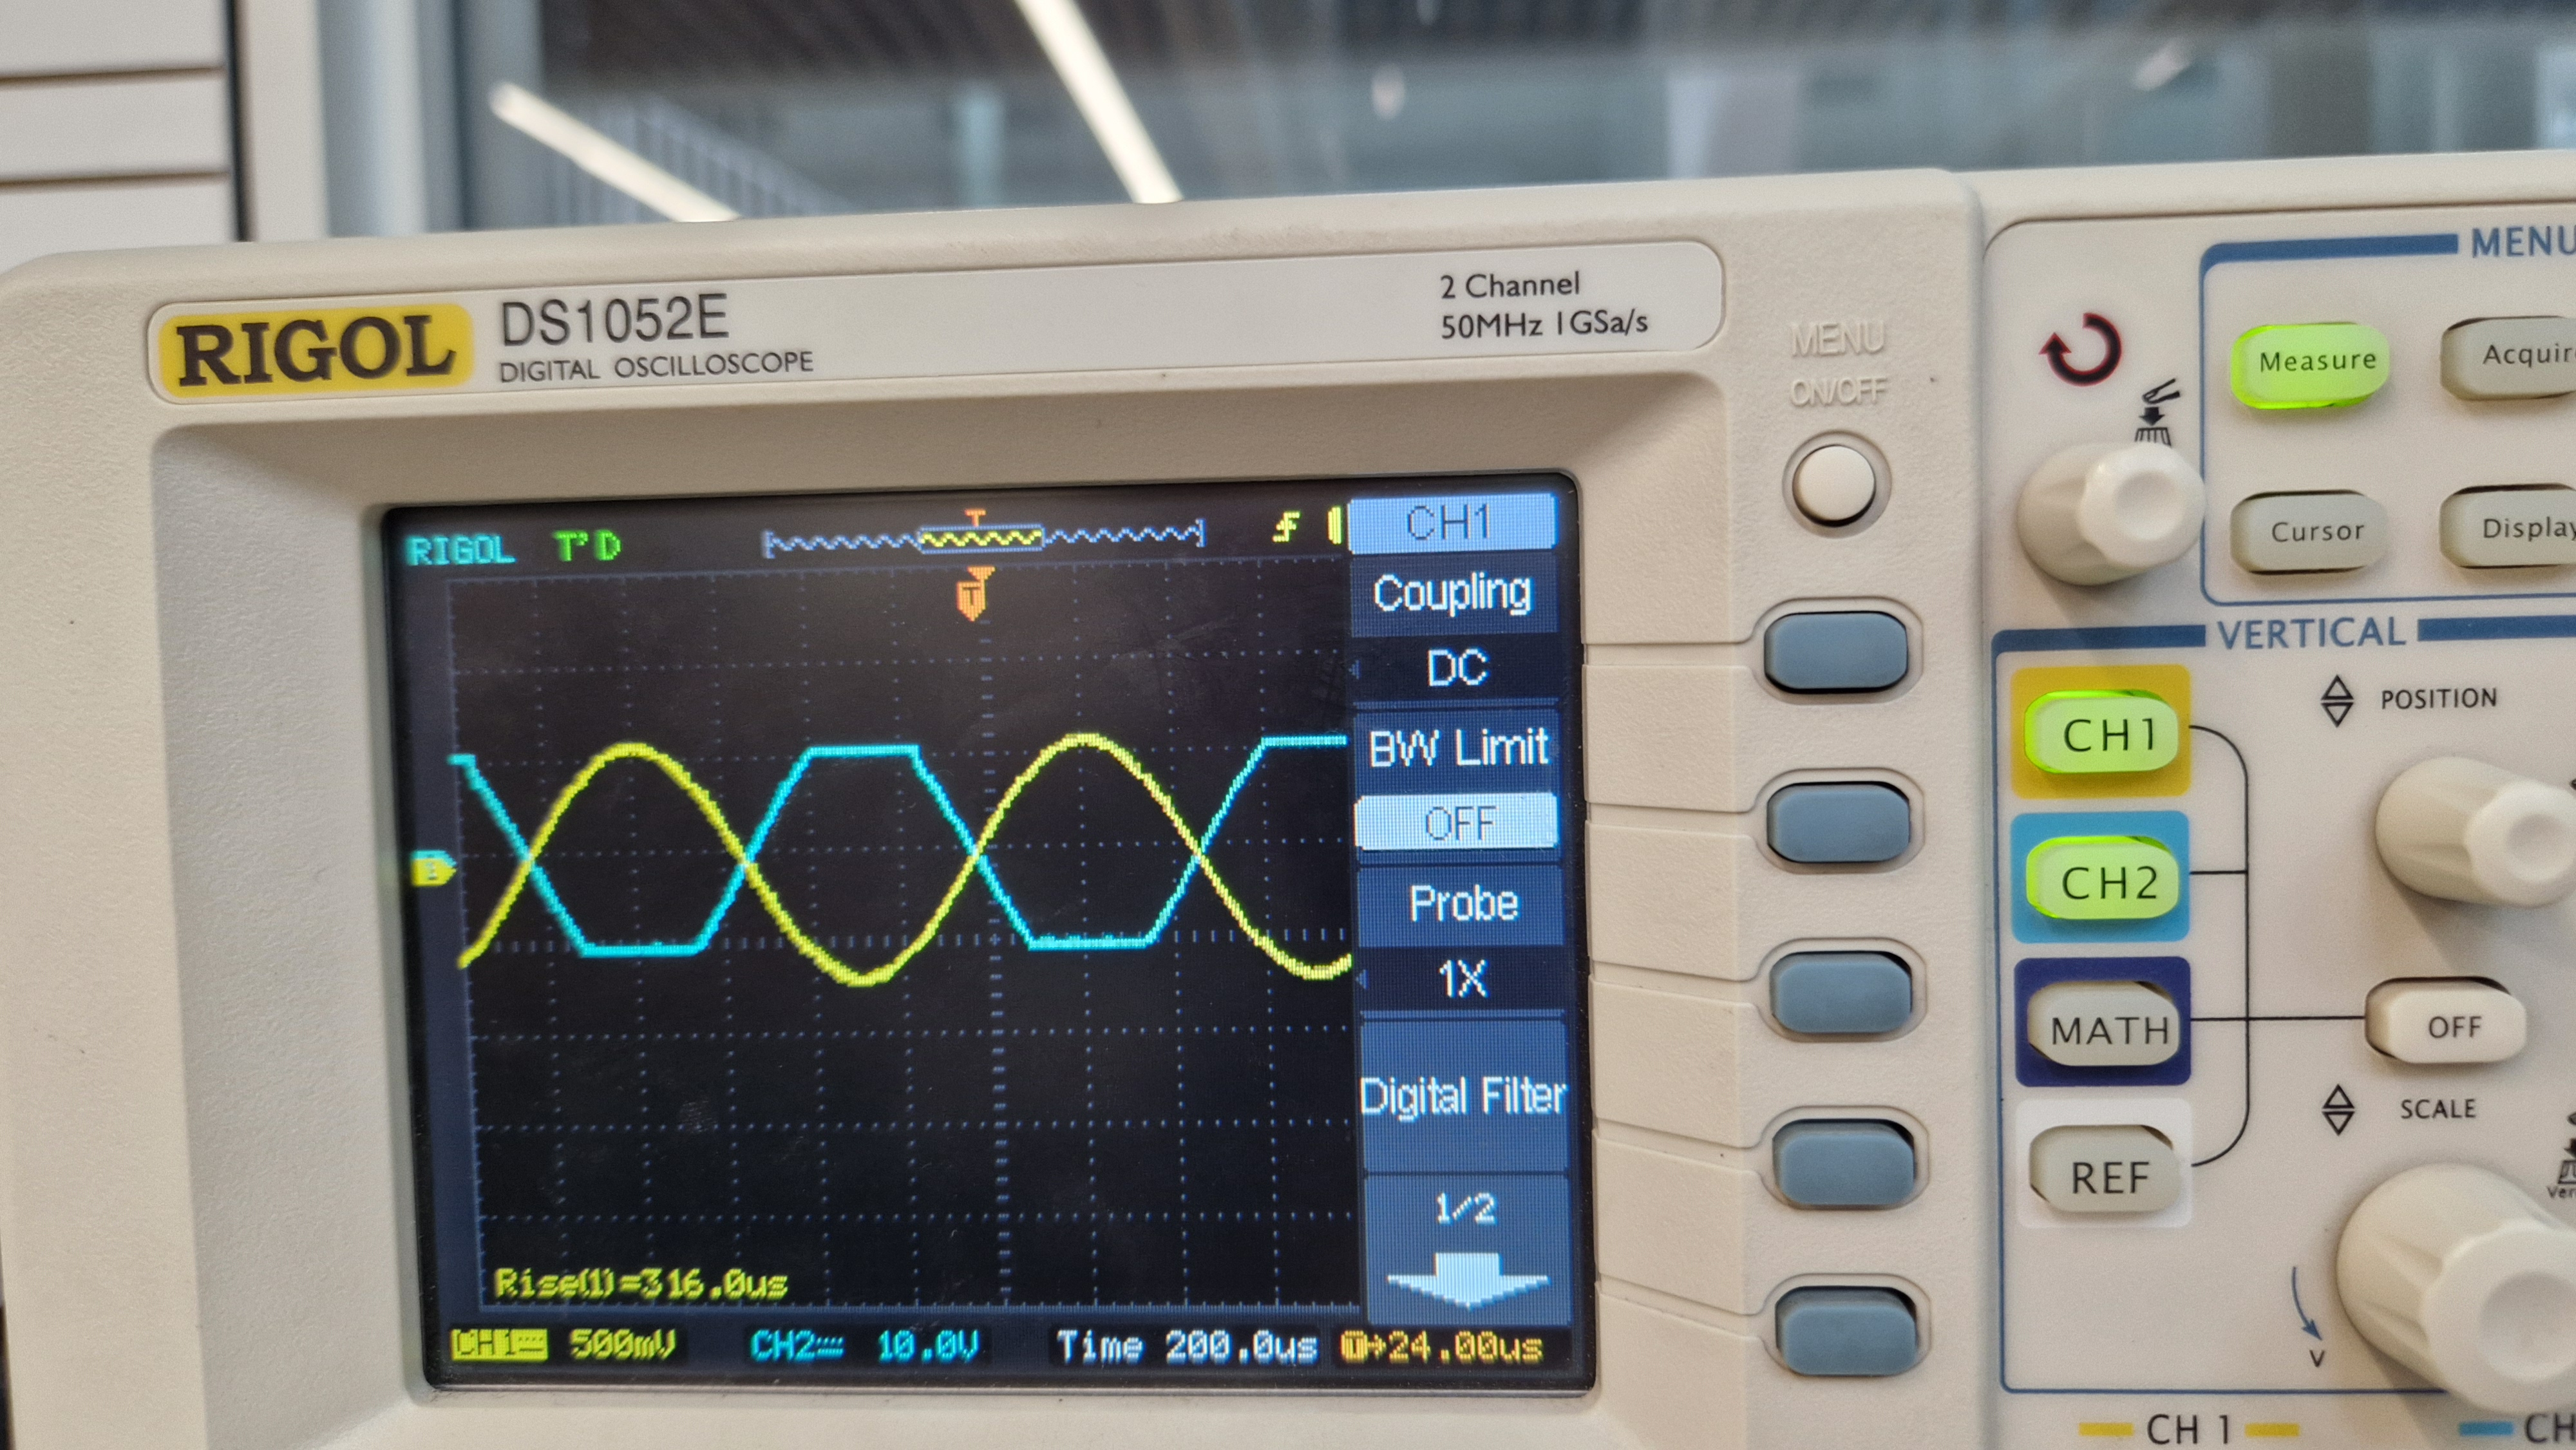
\includegraphics[width=0.6\textwidth]{assets/inverting-1.3-output.jpg}
    \caption{Inverting @ 1.3V}
    \label{fig:inverting-1.3-output}
\end{figure}

Applying 1.3V input to the inverting amplifier, the output should be -28.6V but it is limited to -12V due to the power supply as seen in Figure \ref{fig:inverting-1.3-output}.

\newpage
\thispagestyle{plain}

\begin{figure}[h]
    \centering
    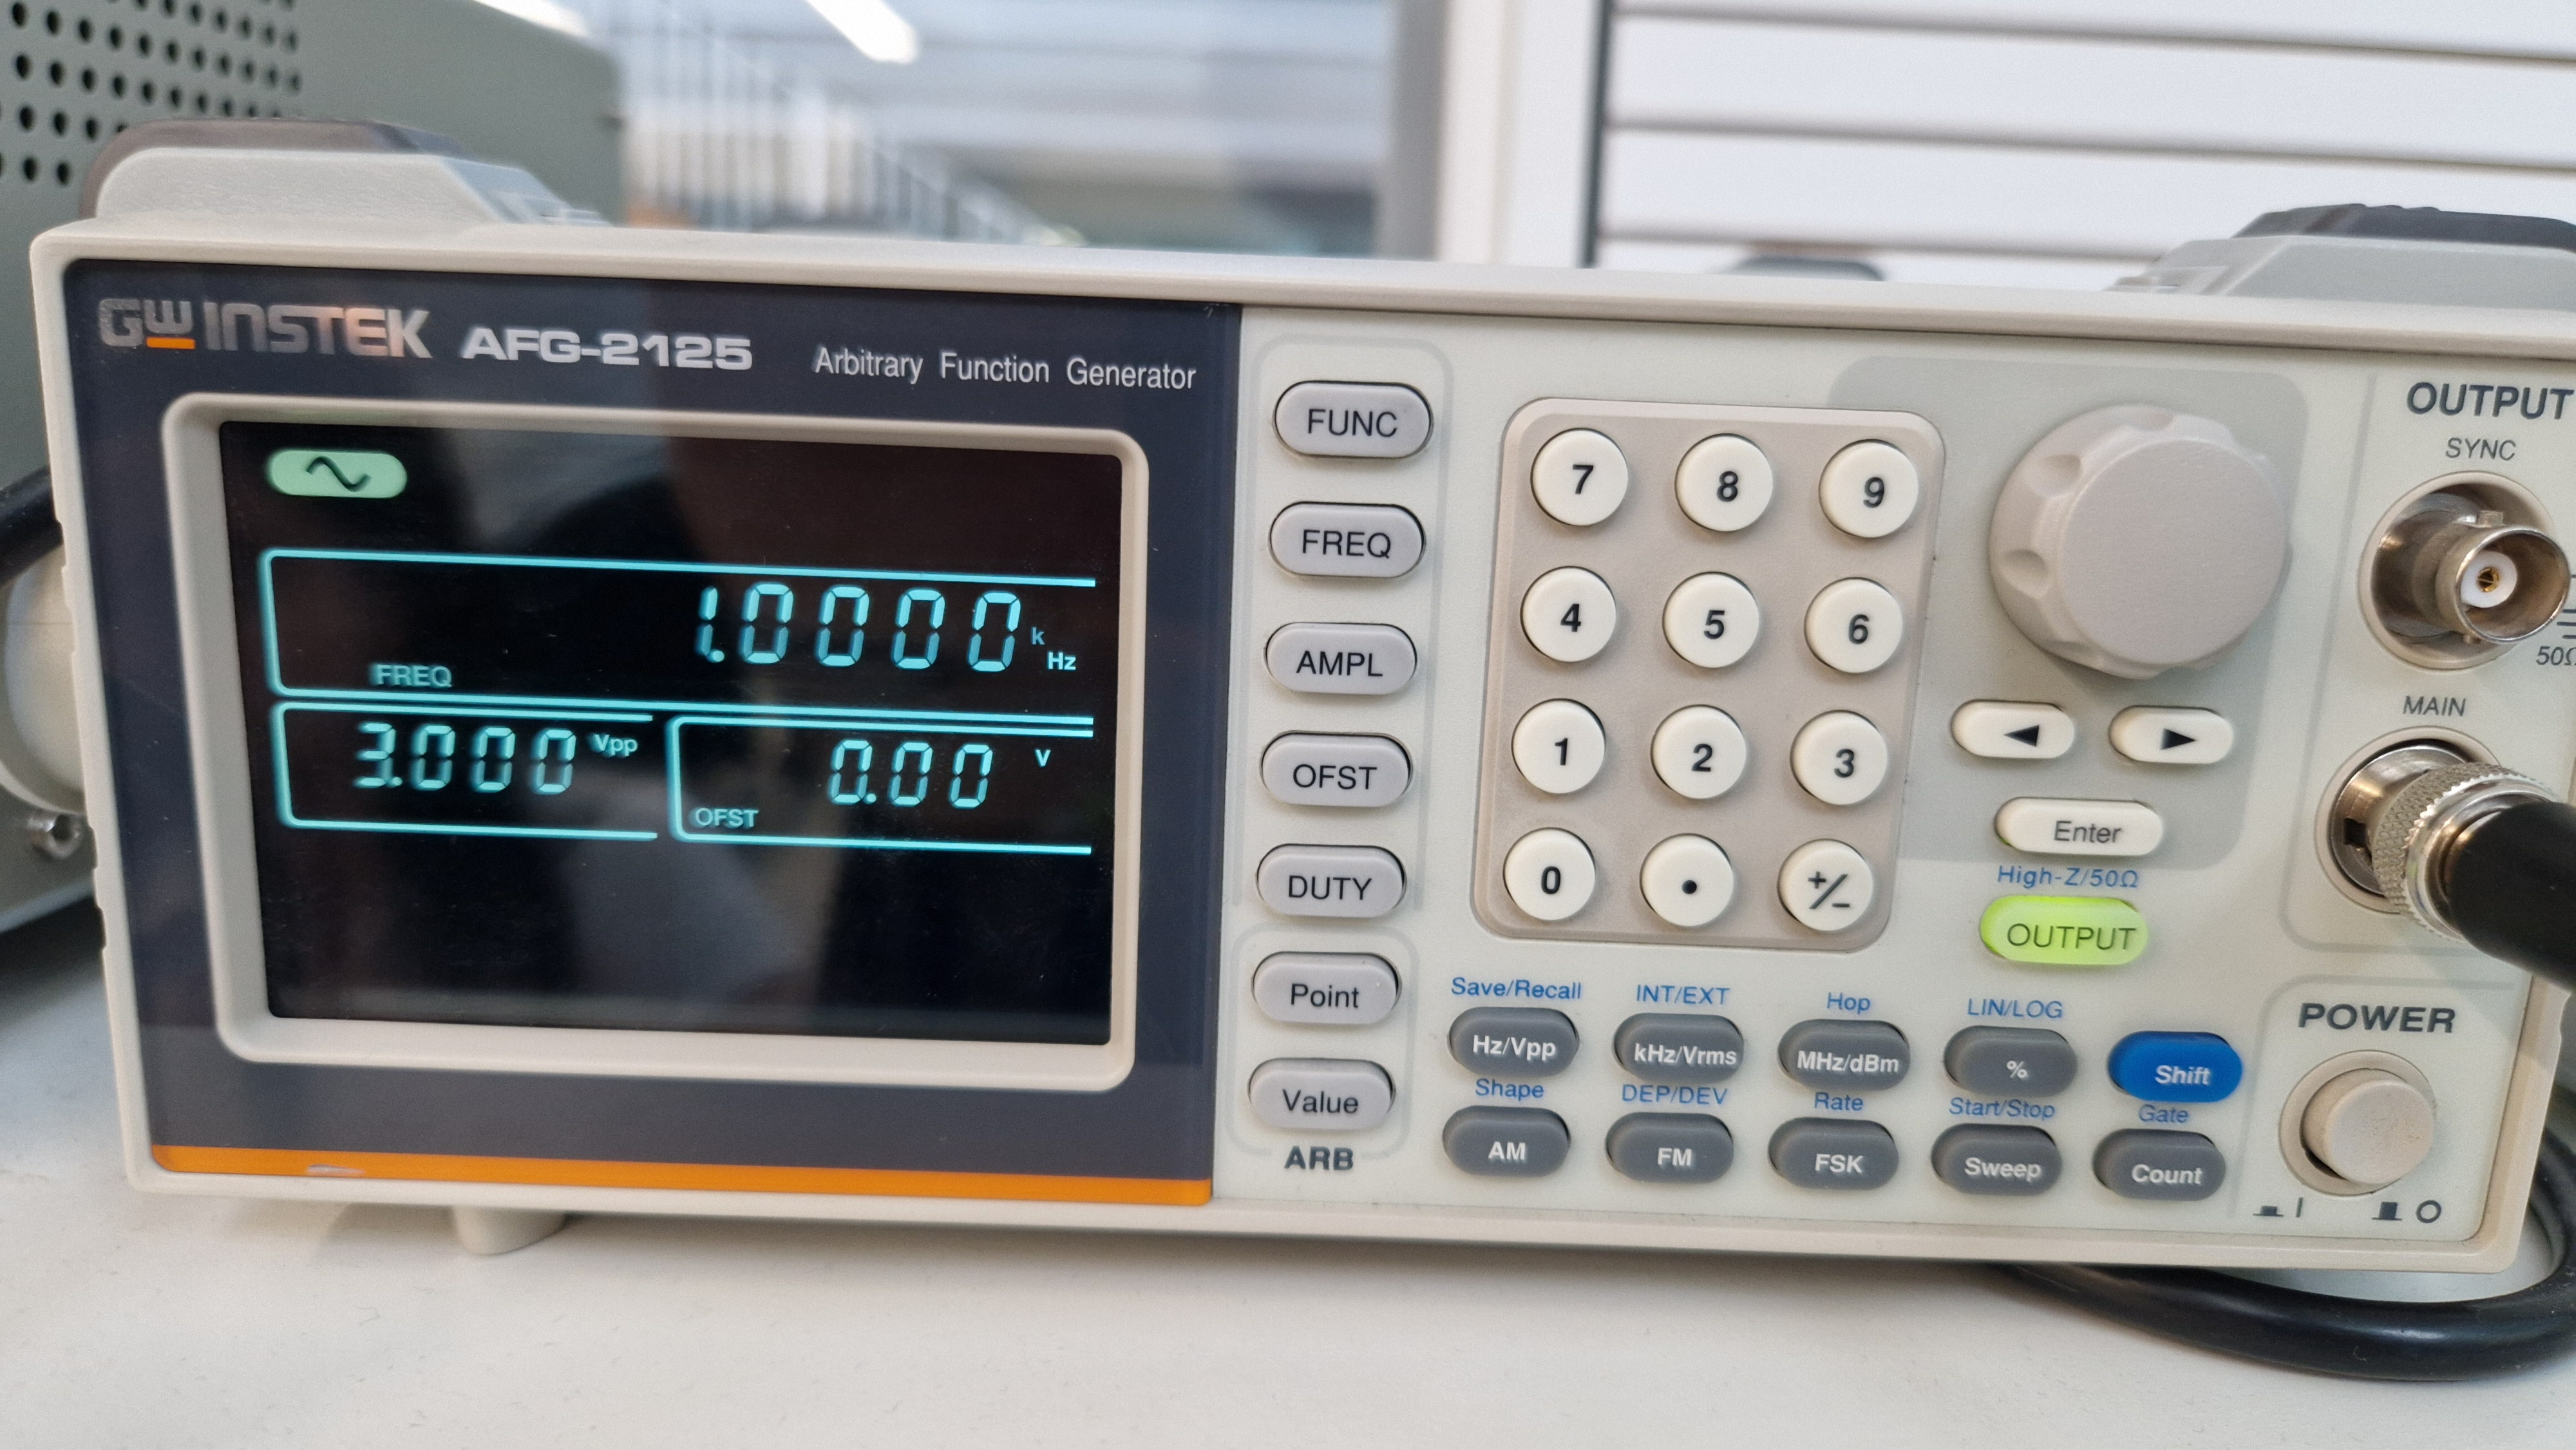
\includegraphics[width=0.6\textwidth]{assets/inverting-3.jpg}
    \caption{Signal Generator @ 3V}
    \label{fig:inverting-3}
\end{figure}

\begin{figure}[h]
    \centering
    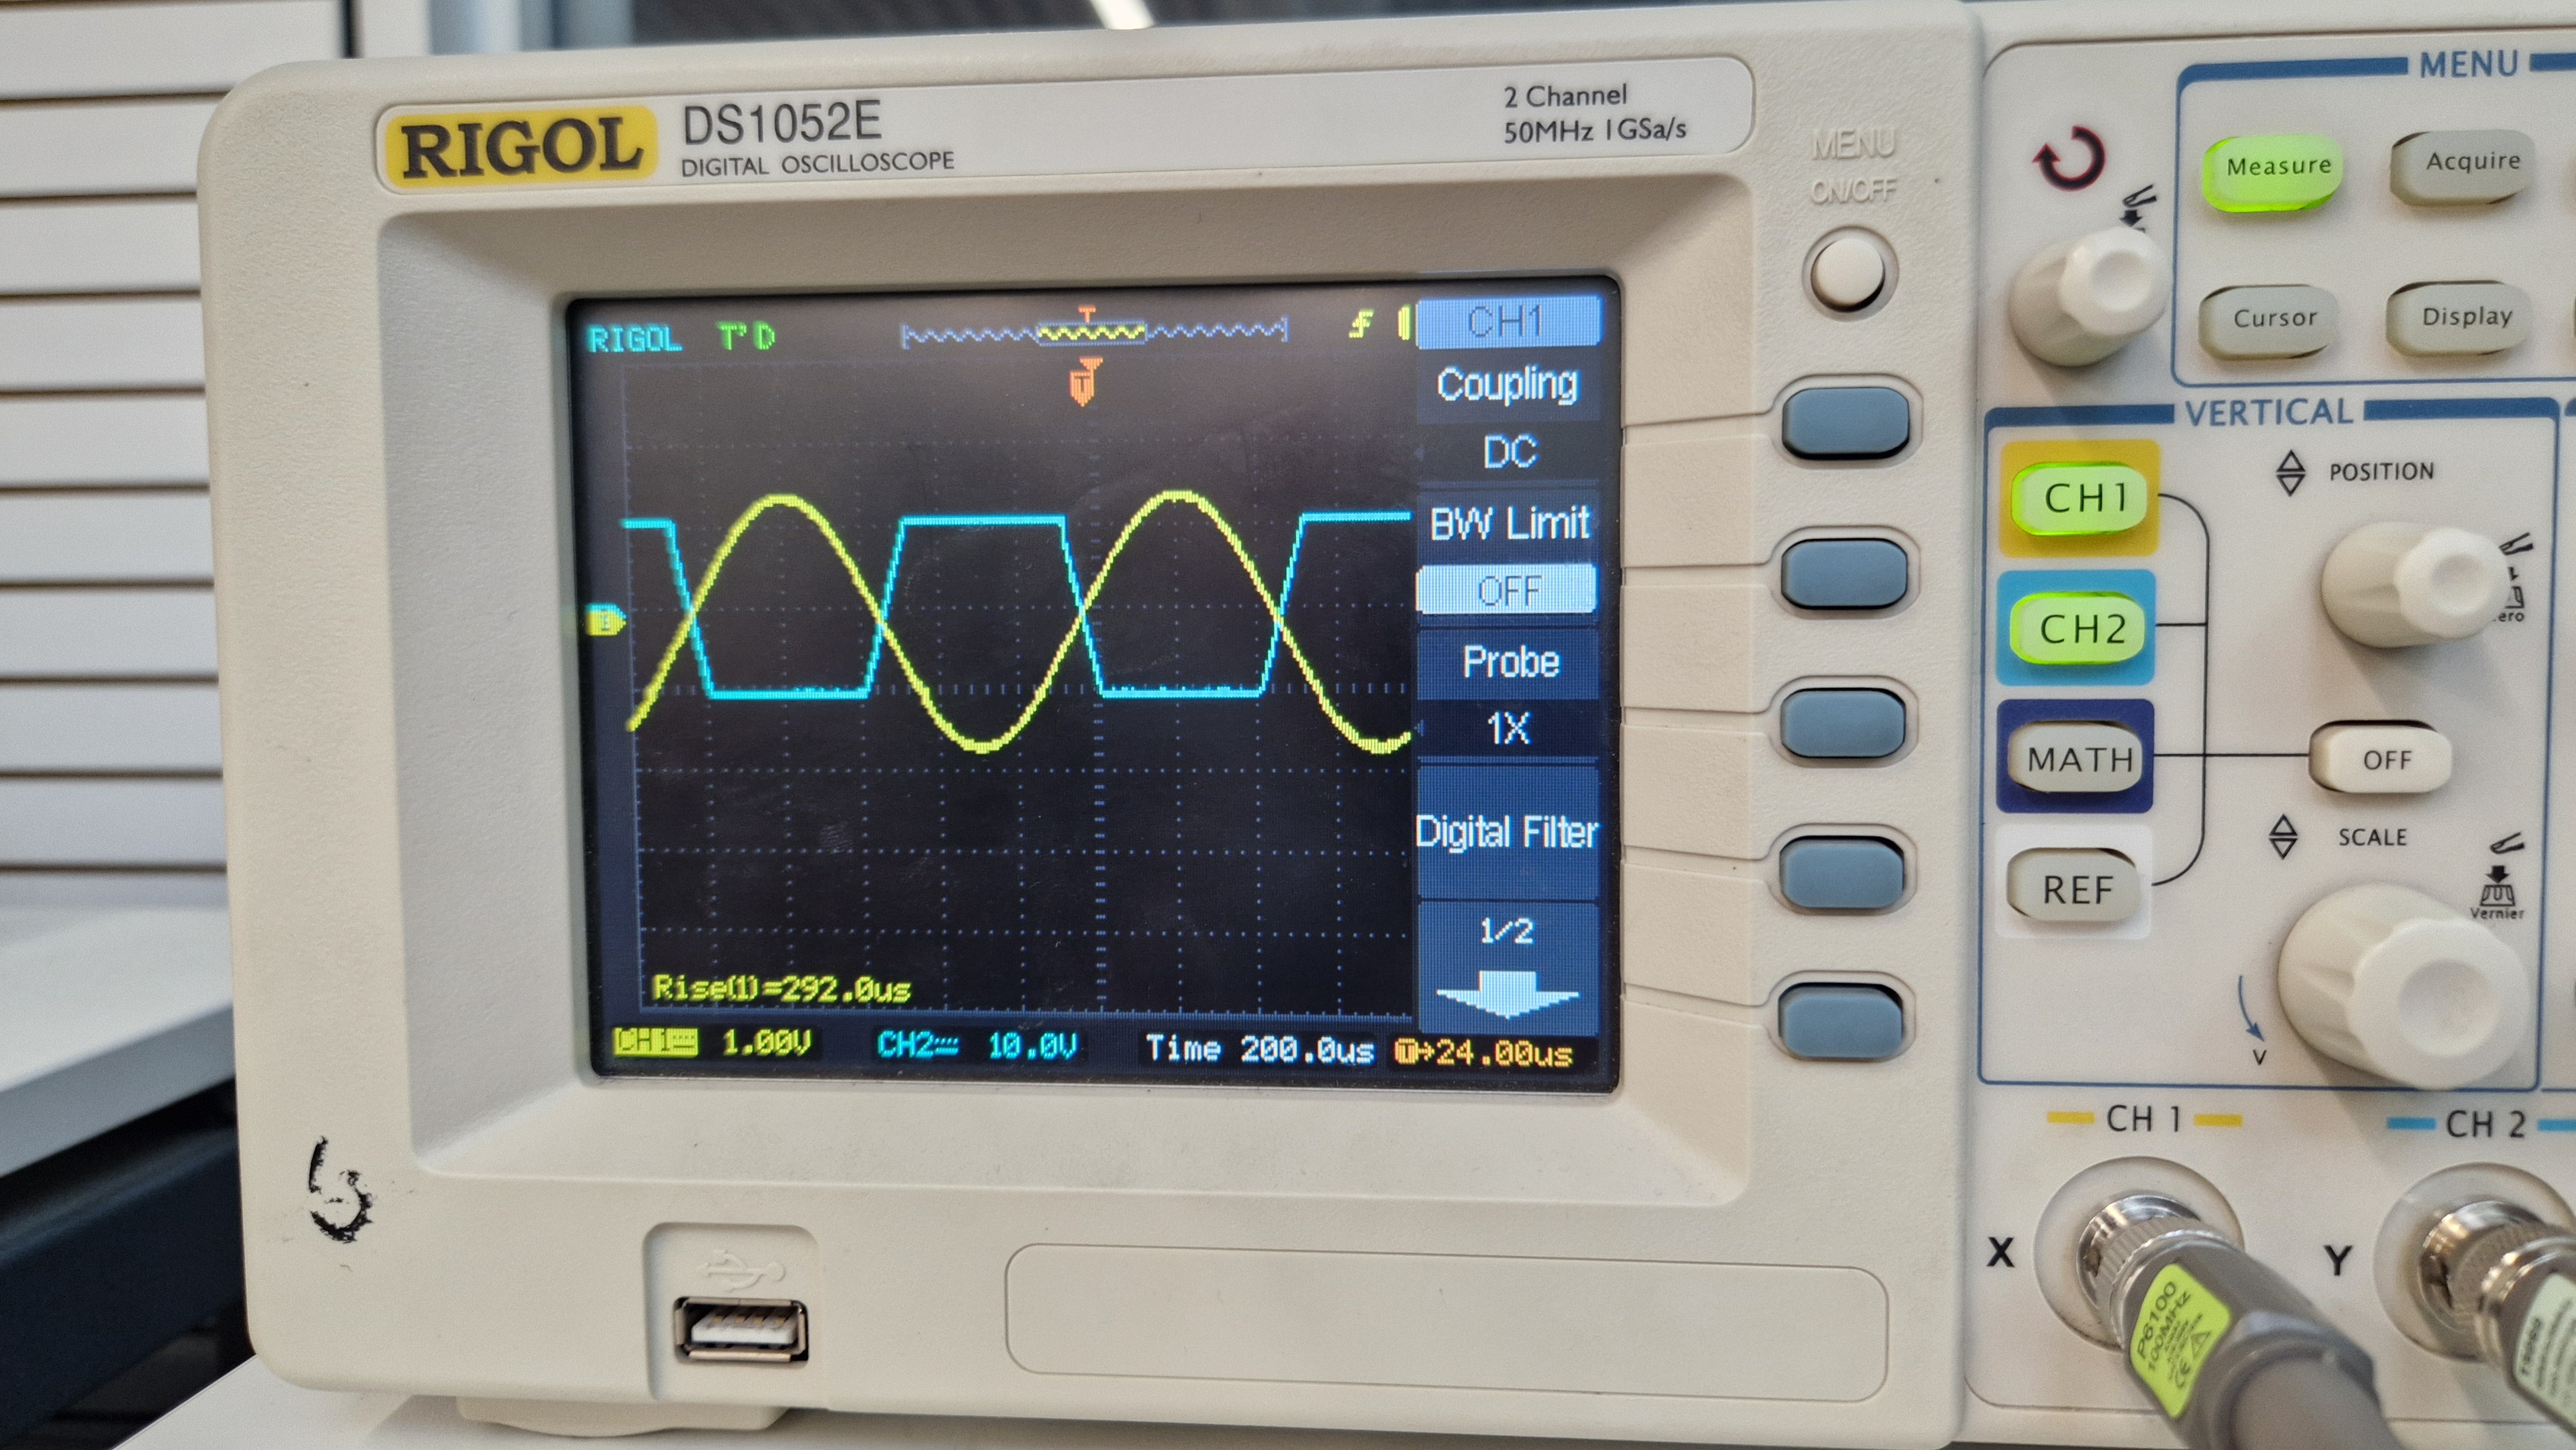
\includegraphics[width=0.6\textwidth]{assets/inverting-3-output.jpg}
    \caption{Inverting @ 3V}
    \label{fig:inverting-3-output}
\end{figure}

Applying 3V input to the inverting amplifier, the output should be -66V but it is limited to -12V due to the power supply as it is \textbf{more visible} in Figure \ref{fig:inverting-3-output}.

	\chapter{Analysis \& Discussions}

\section{Clipping Behavior}

Clipping occurs when the output voltage reaches the supply voltage limits and can no longer increase linearly with the input signal, resulting in a distorted waveform. This is evident in the experimental results where the output voltage is limited to 12V due to the power supply, as seen in Figure \ref{fig:non-inverting-970m-output} and Figure \ref{fig:non-inverting-2-output}. The output voltage should be 13.7V and 23V for 970mV and 2V input signals, respectively. The clipping behavior is more visible in Figure \ref{fig:non-inverting-2-output} due to the higher input voltage.

\section{Theoretical vs. Experimental Results}

The theoretical analysis of the non-inverting amplifier predicts the output voltage to be 2.3V, 13.7V, and 23V for 100mV, 970mV, and 2V input signals, respectively. However, the experimental results show that the output voltage is limited to 12V due to the power supply. This discrepancy between the theoretical and experimental results can be attributed to the limitations of the power supply and the non-ideal behavior of the op-amp.

\section{Simulation vs. Experimental Results}

The simulation results closely match the theoretical analysis, as the simulation software does not have the limitations of the power supply and can accurately model the behavior of the op-amp. In contrast, the experimental results deviate from the theoretical analysis due to the limitations of the power supply and the non-ideal behavior of the op-amp. The simulation results provide a more accurate representation of the expected output voltage for different input signals.

	\chapter{Conclusion}

In this laboratory work, we explored the fundamental characteristics and behavior of Operational Amplifiers (Op-Amps) through theoretical analysis, LTspice simulations, and practical experiments. Our primary objectives were to understand the voltage gain of Op-Amp circuits, observe the input and output voltage waveforms, and analyze the clipping phenomenon.

\section{Key Findings}

\subsection{Theoretical Analysis}

The theoretical calculations for the voltage gain of an inverting and non-inverting amplifier were verified. We found that the expected voltage gain matched the formula \( A_v = 1 + \frac{R2}{R1} \) for the non-inverting configuration and \( A_v = -\frac{R2}{R1} \) for the inverting configuration. For our circuit with \( R1 = 100\Omega \) and \( R2 = 2.2k\Omega \), the calculated gain was 23 for the non-inverting amplifier and -22 for the inverting amplifier.

\subsection{LTspice Simulations}
The LTspice simulations successfully validated our theoretical predictions. The simulated output voltage closely aligned with the calculated values, demonstrating the accuracy of our theoretical analysis. The input and output waveforms were appropriately labeled and matched the expected sinusoidal shapes.

\subsection{Laboratory Exercises}
In the practical implementation, we observed the input and output voltages using an oscilloscope. The experimental results were consistent with both the theoretical and simulated data, confirming the expected voltage gain.

We identified the point of clipping by gradually increasing the input voltage amplitude. The maximum input voltage before clipping occurred was recorded, and the output waveform showed the expected distortion once the Op-Amp reached its supply voltage limits.

\section{Observations \& Analysis}

\subsection{Clipping Phenomenon}
Clipping occurs when the output voltage of the Op-Amp reaches its maximum or minimum limits, resulting in a flat-topped waveform instead of a smooth sinusoidal shape. This happens because the Op-Amp cannot produce an output voltage beyond its supply voltage.

\subsection{Measurement Accuracy}
Our measurements were accurate and closely matched the theoretical and simulated results. Minor discrepancies could be attributed to practical limitations such as component tolerances and measurement errors.

\section{Learning Outcomes}

This lab exercise enhanced our understanding of Op-Amps, specifically how they amplify signals and the conditions under which they operate linearly versus non-linearly (clipping).

We gained practical skills in building and testing electronic circuits, using LTspice for circuit simulations, and accurately measuring and interpreting waveform data with an oscilloscope.

In summary, the laboratory work provided a comprehensive insight into the operational principles of Op-Amps. It highlighted the importance of combining theoretical knowledge with practical skills to analyze and interpret circuit behavior effectively. The successful completion of this lab reinforces the foundational concepts essential for advanced electronic system design.


	\chapter{Appendices}

\section{LTspice Simulation Code}

\subsection{Non-Inverting Amplifier}

\begin{lstlisting}
* Non-Inverting Amplifier @ 100mV 1kHz sine
XU1 N004 N002 N001 N005 N003 LM741
R1 0 N002 1k
V1 N004 0 SINE(0 1 1k)
R2 N003 N002 22k
V2 N001 0 12
V3 0 N005 12
.tran 1m
.lib LM741.lib
.backanno
.end
\end{lstlisting}


\subsection{Inverting Amplifier}

\begin{lstlisting}
* Inverting Amplifier @ 100mV 1kHz sine
XU1 0 N002 N001 N005 N003 LM741
V1 N004 0 SINE(0 1 1k)
V2 N001 0 12
V3 0 N005 12
R1 N002 N004 1k
R2 N003 N002 22k
.tran 1m
.lib LM741.lib
.backanno
.end
\end{lstlisting}


\end{document}
